\documentclass[11pt]{article}
\usepackage[top=2.54cm, bottom=2.54cm, left=2.54cm, right=2.54cm]{geometry}
\linespread{1.5}
\setlength{\parindent}{0cm}
\usepackage{amsmath}
\usepackage{amssymb}
\usepackage{amsthm}
\usepackage{datetime}
\usepackage{graphicx}
\usepackage{float}
\usepackage{tikz}
\usepackage{pgfplots}
\usepackage{hyperref}
\usepackage{subcaption}
\usepackage{bm}
\usepackage{dsfont}
\usepackage{xcolor}
\usepackage{fancyhdr}
\usepackage[labelfont=bf]{caption}

\pagestyle{fancy}
\fancyhf{}
% \rhead{\leftmark} 
\cfoot{\thepage}
\renewcommand{\headrulewidth}{0pt}

\bibliographystyle{ieeetr}
\usepackage{bibentry}
\nobibliography*

\newcommand{\vd}{\mathrm{d}} %Vertical d (for derivatives)
\newcommand{\bmat}[1]{\bm{\mathrm{#1}}}
\newcommand{\bvec}[1]{\bm{\mathrm{#1}}}
\newcommand{\grad}{\bvec{\nabla}}

\begin{document}
	\pagenumbering{arabic}
	
	\begin{titlepage}
		\begin{center}
			
			\vspace{0.025\textheight} % Whitespace between the top rules and title
			
			{\huge \textbf{Modelling the Cooking of Steak through Finite Difference Methods}}\\[0.3cm]
			
			{\Large BSc Dissertation}
			
			\vspace{0.025\textheight} % Whitespace between the title and short horizontal rule		
			\rule{0.3\textwidth}{0.4pt} % Short horizontal rule under the title
			\vspace{0.025\textheight} % Whitespace between the thin horizontal rule and the author name
			
			Tavis O'Reilly (10903943)\\[0.3cm]
			\textit{Department of Physics and Astronomy}\\[0.3cm]
			\textit{The University of Manchester}\\[0.3cm]
			\shortmonthname[\the\month]  \the\year \\[2cm]
			
		\end{center}
		
		\vspace{0.1\textheight} % Whitespace between the thin horizontal rule and the author name
		
		{\Large \textbf{Abstract}}\\
		
		There are many qualitative descriptions of the cooking methods that give a "perfect" steak, but little quantitative analysis to back this up. In this dissertation, using finite difference solutions to the heat equation, I simulated the diffusion of heat throughout a steak for four different cooking methods. I then measured the values of three criteria (the amount of Maillard reaction products, the evenness of the cook, and the skew of the cook) to quantify the quality of each cooked steak. My findings were that a reverse searing method (cooking in a low temperature oven first, followed by a quick sear in a hot pan) was the best method based on all of my metrics. It gave a larger amount of Maillard reaction products, the most even cook, and a cook that wasn't skewed to either side.
		
		\vfill
	\end{titlepage}
	
	\pagenumbering{gobble}
	\clearpage
	\pagenumbering{arabic}
	\setcounter{page}{2}
	
	\newpage
	
	\section{Introduction}
	
	The goal of this dissertation will be to model and compare different methods that can be used to cook a beef steak. Beef is a widely-eaten meat around the world; the highest-meat-consuming country -- the USA, ate 38.01 kg of beef per capita, in 2022 alone\cite{beef_consumption}. A beef steak is a simple and popular way to enjoy this beef, so perfecting the cooking method -- maximising the flavours, and quality of texture, is an important topic to consider. \\
	
	There are many anecdotal descriptions from various chefs around the world about the cooking method that gives the "perfect" steak: Gordon Ramsay goes with a simple pan sear on high heat, with a good resting period afterwards\cite{ramsay_steak}; Heston Blumenthal is a fan of rapidly flipping his steak (every 15 seconds) while cooking on a hot pan\cite{heston_steak}; and Kenji L\'opez-Alt goes for a reverse sear method -- cooking the steak low and slow, followed by a quick high-temperature sear\cite{kenji_steak}. To make an informed decision about which method is the best, there is a need to quantify the criteria that define a well-cooked steak, and then to use these criteria to evaluate and compare each different method. \\
	
	All cooking methods have something in common -- the transfer and diffusion of heat throughout the steak. This heating is applied such that the steak reaches a certain "doneness" level, determined by the internal temperature (these levels and their respective temperatures are outlined in \autoref{tab:doneness}). Where the differences lie is in the path taken by the temperature at each point in the steak; determining whether, and for how long, they reach certain critical temperatures where different physical or chemical processes can occur. Some of these changes may be desirable, for example developing a brown crust, and some may be less so; for example toughening of the meat or even burning of the outside. \\
	
	In this dissertation, I will research and decide upon the key criteria that are found in a good steak. I will then construct a computational model of the heat diffusion that occurs during cooking, and use this to quantify each of my criteria. Hopefully determining a "best" method overall.
	
	\begin{table}[H]
		\centering
		\begin{tabular}{|c|c|}
			\hline
			Doneness Level & Internal Temperature \\
			\hline
			Rare & 120 $^\circ\text{F}$ / 49 $^\circ\text{C}$ \\
			Medium-Rare & 130 $^\circ\text{F}$ / 54 $^\circ\text{C}$ \\
			Medium & 140 $^\circ\text{F}$ / 60 $^\circ\text{C}$ \\
			Medium-Well & 150 $^\circ\text{F}$ / 66 $^\circ\text{C}$ \\
			Well-Done & 160 $^\circ\text{F}$ / 71 $^\circ\text{C}$ \\
			\hline
		\end{tabular}
		\caption{A set of internal temperatures corresponding to each "doneness" level. These are one set of values\cite{doneness}. Although there is a general consensus on the approximate temperature ranges, there are no exact values, and sources vary.}
		\label{tab:doneness}
	\end{table}
	
	\section{Literature Review}
	
	Before delving into my own modelling and research, I will summarise some key parts of existing literature on the subjects of modelling the cooking of meat, the Maillard reaction, and properties of meat proteins. The literature is generally less evaluative than my dissertation will be, instead aiming to calculate cooking times from the models, however there is significant overlap in the methods I need to produce my own model for the cooking of a steak. I will be able to use the information from this literature to inspire the direction of my work.
	
	\subsection*{Modelling of Turkey Cooking}
	
	The first paper I would like to discuss is a paper by Jin et al.\cite{turkey_2021}, investigating the relationship between the size of a turkey and the time it takes to cook. This built upon an empirical formula -- the Panofsky formula, and attempted to theoretically derive the basis for this formula. This has the general overlap that it models the cooking of meat in an oven -- something I will need for simulating certain cooking methods. In their modelling, they approximate the shape of a turkey as spherical. This is a decent (and useful) approximation for a turkey, but for a steak, a cuboidal shape will be more beneficial. \\
	
	They aim to solve the heat equation in one dimension (the radial direction), with the simple boundary conditions of all points beyond the radius of the sphere being at a fixed temperature $T=T_h$, where $T_h$ is the temperature of the oven. The boundary conditions are an oversimplification, since the thermal conductivity (among other properties) changes at the boundary, and it completely neglects the convection that takes place in air. While it may work for their case, I will need to use an improved boundary condition for contact with air, taking into account the full convective heat transfer. \\
	
	Their solution is also analytic; for modelling cooking methods which involve many parameters changing, computational modelling will be much more convenient.
	
	\subsection*{Modelling Meat Cooking by Finite Elements}
	
	This next paper by Purlis et al.\cite{meat_cook_finite_elements} models the cooking of a meat roast in an oven, using a similar finite differences method to what I intend to use. They couple both the heat equation, and diffusion equation to model the combined mass and heat transfer. They also modelled a full 3-dimensional mesh for the bounds of the problem. These are both slightly beyond what I will be doing, instead modelling in a single dimension, and considering only the heat equation, but there are still valuable things to be learned from this method. \\
	
	Their meat-air boundary condition made use of Newton's law of cooling to model convective heat transfer, something that was missing from the previous paper. I can take this on board for my modelling of cooking in an oven, and the air boundary when cooking in a pan.
	
	\subsection*{Thermophysical Properties of Meat}
	
	An important aspect of accurately modelling the diffusion of heat in a steak is to have a value for its thermal diffusivity; that is the subject of this next paper by Marcotte et al.\cite{meat_diffusivity}. They investigate the thermal conductivities, densities, and heat capacities of various types of meat as a function of temperature. Combining these give the thermal diffusivity, which they graphed as a function of temperature, finding that the values ranged between $1\text{-}1.5 \times 10^{-3}\;\mathrm{cm}^2\mathrm{s}^{-1}$. Starting on the lower end of the range at room temperature. While none of the meats tested were beef specifically, it showed that the meats tested do not differ significantly in the order of magnitude for their thermal diffusivity values. \\
	
	There are other factors to consider beyond using a single value for the thermal diffusivity of meat. As already discussed, the value depends on temperature, but not only that, meat is not homogeneous and so heat will diffuse differently depending how the meat is cut. To avoid these complexities, I will use a single temperature-independent value as an approximation.
	
	\subsection*{Reverse Sear vs. Oven Cooked Steak}
	
	A key paper relating to my criteria (by Yoo et al.\cite{steak_sear}) evaluates "the sensory and instrumental quality" of steak cooked with a reverse sear (oven cooked followed by a quick, hot pan sear) and steak cooked only in an oven. The key finding was that although key properties such as water content were not affected, there was a noticeable increase in products of the Maillard reaction\footnote{The Maillard reaction is a series of chemical reactions that take place at high temperatures (>140-165 $^\circ\text{C}$); it converts amino acids and reducing sugars into flavourful compounds known as melanoidins. This is discussed further in \autoref{maillard_reaction}.} in the steak that was seared at high temperature. When the flavour of the steaks were rated by participants of the study, those that were seared scored much higher. The conclusion formed was that the flavour was improved solely due to these Maillard reaction products. \\
	
	Ensuring the Maillard reaction takes place on the surface of a steak is clearly an important factor in determining the quality of the cooking method. I will use this as one of my key criteria to measure from the model.
	
	\subsection*{Computational Modelling of Cooking Steak}
	
	The final paper by Moya et al.\cite{steak_modelling} is closest in terms of modelling to what I am intending to do. They use a similar finite differences method to Purlis et al., including the coupling of the heat and diffusion equations. They also factor in the water holding capacity of the proteins in the meat, to include a "dripping factor", and including the latent heat of vaporisation into their calculations. The diffusion of water, how it interacts with proteins in the meat, and its vaporisation, are all important things to consider alongside heat flow. \\
	
	The results of the model were compared to experimental data, and matched extremely closely, giving estimated cooking times for various "doneness" levels of a steak cooked on both sides in a pan. While my model will not be this detailed, I can use the data from their model to compare my results with, and use elements of their model, such as basic water vaporisation modelling, in my own work.
	
	\subsection{Summary}
	
	There are many papers investigating and building models for the important process of heat and moisture transfer during cooking. Having good models is crucial for producing cooking guides on a range of foods, but specifically meats. The models range from very basic analytic solutions (which still give useful results) to complex computational models including heat transfer, moisture transfer, and more. I intend to produce a model somewhere in the middle of these that I will then be able to use to compare, and form conclusions about, various methods of cooking a steak.
	
	\section{Theory}
	
	I will now discuss the key areas of theory that will be required to analyse the different steak cooking methods.
	
	\subsection{The Heat Equation}
	
	When cooking a steak, the key process governing how its temperature profile changes over time is the conduction of heat. This is described by the heat diffusion equation\cite{heat_equation}
	\begin{equation}
		\frac{\partial T}{\partial t} = \alpha \nabla^2 T,
	\end{equation}
	where $T \equiv T(\bvec{r}, t)$ is the temperature field over space, $t$ is time, and $\alpha$ is the thermal diffusivity of the medium. For meat, the thermal diffusivity varies based on many factors (including temperature), but it is approximately in the range $1\text{-}2 \times 10^{-3}\;\mathrm{cm}^2\,\mathrm{s}^{-1}$\cite{meat_diffusivity,meat_diffusivity2}. I will use the midpoint of this range for my model.\\
	
	Solving this equation requires two things: an initial temperature field $T_0(\bvec{r})$, which defines the temperature the steak begins at, when $t=0$; and a set of boundary conditions that define how heat is transferred between the steak and its surroundings. For my cooking methods there will be two main boundary types: a steak-pan boundary, and a steak-air boundary. \\
	
	For the steak-pan boundary, I will use a so-called Dirichlet boundary condition, fixing the temperature to be $T(x=0) = T_p$, where $T_p$ is the temperature of the pan. For the steak-air boundary, I will use a so-called Neumann boundary condition, fixing the spacial derivative of the temperature. This is related to the heat flux $\bvec{q}$ by\cite{heat_equation}
	\begin{equation}
		\bvec{q} = \kappa \grad T,
	\end{equation}
	where $\kappa$ is the thermal conductivity, related to the thermal diffusivity $\alpha$ by
	\begin{equation}
		\alpha = \frac{\kappa}{\rho c},
	\end{equation}
	where $\rho$ is the density, and $c$ is the specific heat capacity. \\
	
	At a boundary with air, the convective heat transfer can be modelled with Newton's law of cooling\cite{convection}
	\begin{equation}
		q_\perp = h(T - T_\infty),
	\end{equation}
	where $q_\perp$ is the heat flux out of the surface, $h$ is the heat transfer coefficient, and $T_\infty$ is the temperature of the surrounding air far from the surface. For still air and free convection, the heat transfer coefficient is approximately $h \approx 25\;\mathrm{W}\,\mathrm{m}^{-2}\,\mathrm{K}^{-1}$\cite{heat_transfer_coeff}. \\
	
	With these two boundary conditions, I can vary their associated temperatures and the regions they are applied to in order to model each cooking method, and the cooling/carry-over cooking afterwards.
	
	\subsection{The Maillard Reaction}
	
	\label{maillard_reaction}
	
	The Maillard reaction, first discovered by the French chemist Louis Maillard\cite{maillard}, is a key chemical process that takes place when searing meat (and the cooking of many other foods such as bread) to produce a range of chemical compounds known as melanoidins, that contribute to an improved and deeper flavour. The reaction is between the amino acids and reducing sugars both found in meat, and begins to occur at temperatures around 140-165 $^\circ \text{C}$\cite{maillard_temp}. This will be a key factor in cooking a good steak. The general reaction mechanisms for the Maillard reaction is shown in \autoref{fig:maillard_mechanism}.
	
	\begin{figure}[H]
		\centering
		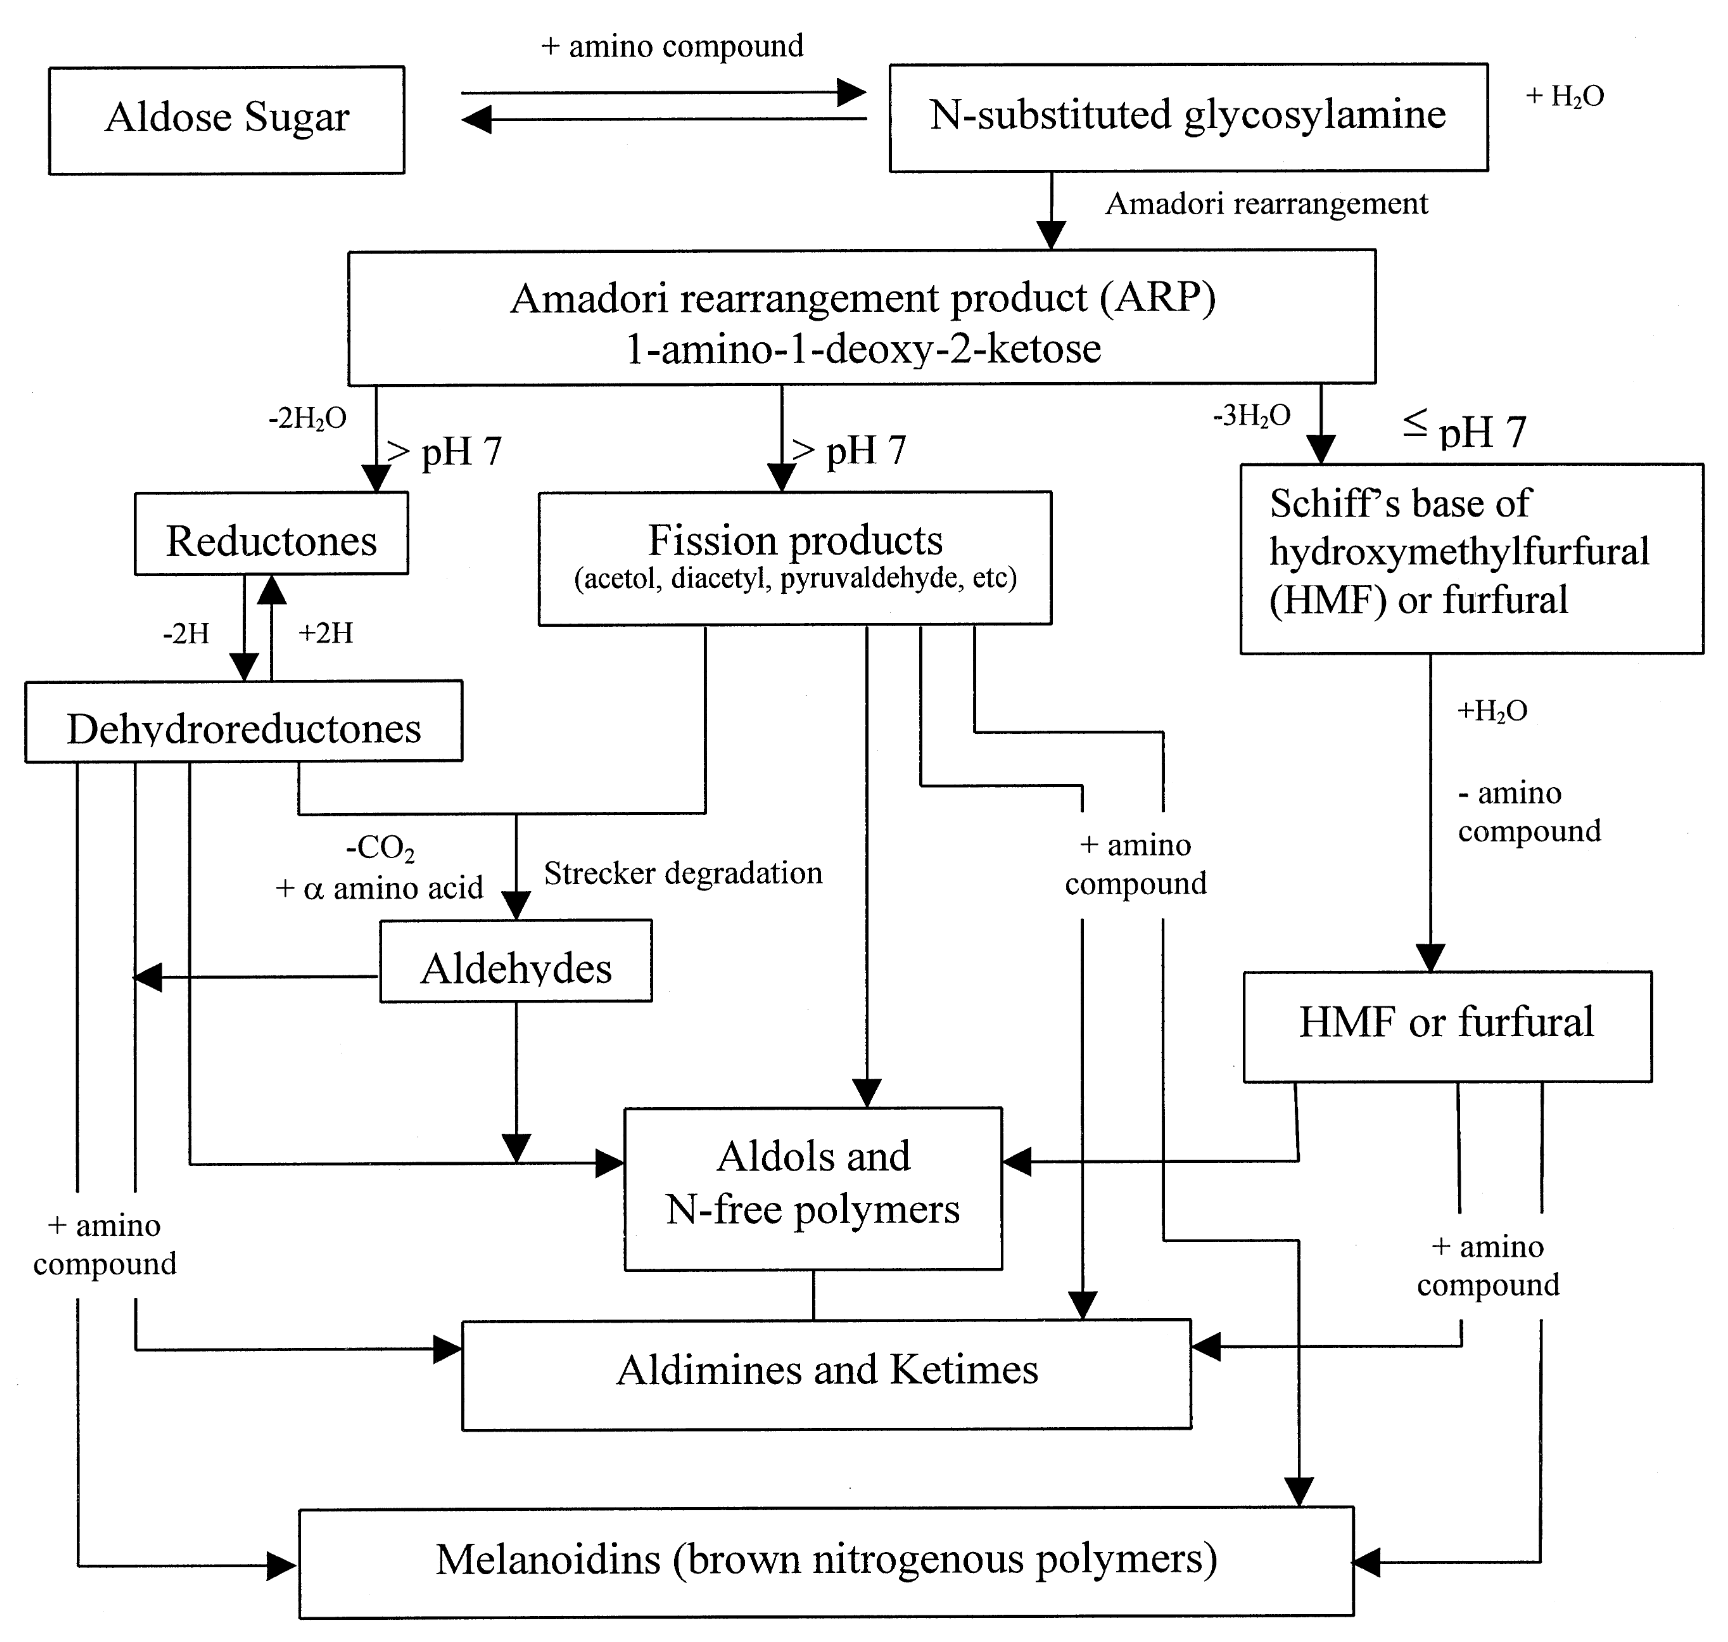
\includegraphics[width=0.8\textwidth]{./img/maillard-mechanism.png}
		\caption{A flowchart diagram showing a general overview of the mechanisms, and their order, involved in the Maillard reaction. Starting with the reducing sugars reacting with amino acids, and ending with melanoidins (in one case). Copied from Martins, Jongen, and van Boekel\cite{maillard_mechanism}; adapted from Hodge\cite{hodge_adapted}.}
		\label{fig:maillard_mechanism}
	\end{figure}
	
	While the Maillard reaction starts to occur at 140-165 $^\circ \text{C}$, it also increases in rate with higher temperatures, as with most chemical reactions. The standard equation describing this is the Arrhenius equation\cite{arrhenius, arrhenius_2}
	
	\begin{equation}
		k \propto \exp{\left(\frac{E_a}{RT}\right)},
	\end{equation}
	where $R$ is the universal gas constant, $T$ is the temperature, and $E_a$ is the molar activation energy for the reaction. For the Maillard reaction, the limiting molar activation energy is approximately $E_a \approx 120\;\mathrm{kJ}\,\mathrm{mol}^{-1}$\cite{maillard_activation}. This corresponds to roughly a doubling of reaction rate with every 10 $^\circ \text{C}$ increase in temperature. \\
	
	At very high temperatures (upwards of 200 $^\circ \text{C}$), pyrolysis of the fat in the steak begins to occur, producing bitter unpleasant compounds such as acrolein\cite{acrolein}. The Maillard reaction also increasingly produces other undesirable compounds such as acrylamide\cite{acrylamide}. For prolonged time at these temperatures, these will overtake, and overpower the desirable flavours from the Maillard reaction. This will be an important thing to avoid; essentially, more Maillard reaction isn't always a good thing.
	
	\subsection{Water Diffusion}
	
	A steak is, by mass, upwards of 70\% water\cite{water_content}, so the role that water and steam plays in the cooking process is important. This is mostly through two processes: vaporisation and diffusion. Water's boiling point is at 100 $^\circ\text{C}$, so when a region of the steak reaches this temperature, the water will vaporise, taking energy away from further temperature increase. The required energy to vaporise 1 kg of water is known as its latent heat of vaporisation $L$. \\
	
	As well as vaporisation, both water and steam will diffuse through the steak fibres following the diffusion equation\cite{diffusion}
	\begin{equation}
		\frac{\partial \phi}{\partial t} = D\nabla^2 \phi,
	\end{equation}
	where $\phi$ is the density of the diffusing material (water or steam in this case), and $D$ is the diffusion coefficient. The steam especially, will flow out from the surface of the steak, transporting energy with it. This change in water content will in turn affect the thermal diffusivity of the steak, making these coupled differential equations. \\
	
	Due to time constraints, I will not be including a full treatment of these processes into my model. So this will be one known source of inaccuracy in the modelling.
	
	\subsection{Texture}
	
	The final key process that occurs during the cooking of a steak is the physical changes to the muscle and connective tissue that make up the meat. Muscle tissue is mainly comprised of the proteins myosin and actin\cite{myosin} along with myoglobin which gives raw steak its red colour\cite{myoglobin}. As temperature increases to around 60 $^\circ\text{C}$ the proteins in this tissue begin to denature\cite{denature}. This causes the meat to soften, giving it a more pleasant texture. \\
	
	When the temperature increases further than this approaching 70 $^\circ\text{C}$, the denatured proteins will then begin to coagulate. This causes the meat to become tougher, and also expel moisture. The balance along this scale gives rise to the different levels of "doneness" for your steak. For the most tender meat, a medium-rare steak is usually best, but since the best level of "doneness" for a steak is quite subjective, I will leave this out of my criteria. Instead focusing on what percentage of the steak reaches the correct desired temperature.
	
	\section{Modelling}
	
	I will only be modelling the temperatures of the steak in one dimension -- the thickness of the steak, since the main surface area is at either end of this axis. There will be small differences between this and a full three-dimensional model, but these are only significant at the edges. Making this simplification makes the modelling less computationally expensive, and also simpler to present. The boundary conditions also become much more simple, as there are only two positions to apply them.\\
	
	\subsection{Computation}
	
	In one dimension, the heat equation simplifies to
	\begin{equation}
		\frac{\partial T}{\partial t} = \alpha \frac{\partial^2 T}{\partial x^2},
	\end{equation}
	where $\alpha$ is the thermal diffusivity. To solve this, I will be dividing the length of the steak into $N_x$ segments of size $\Delta x$, and the time into $N_t$ intervals of length $\Delta t$. The solution to the differential equation can then be approximated by the iterative formula
	\begin{equation}
		T_{i+1}^j = T_i^j + \alpha\Delta t \cdot \frac{T_i^{j+1} - 2T_i^j + T_i^{j-1}}{\Delta x^2},
	\end{equation}
	where $T_i^j$ denotes the temperature on the $i$th time step, at the $j$th position. On each time step, the boundary conditions must be fixed first, either by fixing a temperature value or by fixing the difference between adjacent temperatures to set the derivative. \\
	
	With this iterative formula, one has to be careful of the convergence properties of the solution. Whether the solution converges depends on the CFL condition\cite{cfl_cond}
	\begin{equation}
		C = \frac{\alpha \Delta t}{(\Delta x)^2} \leq \frac{1}{2}.
	\end{equation}
	It will be important to ensure this inequality is satisfied, so that the numerical solution gives sensible results. \\
	
	The final component of my modelling will be to include some limited inclusion of the water content of the steak. I will include the latent heat of vaporisation of water, so that when a region of steak reaches 100 $^\circ\text{C}$, before any further temperature increase, the energy of the latent heat must be met.
	
	\subsection{Measured criteria}
	
	I decided upon the following key criteria to measure, for determining how well the steak is cooked:
	\begin{enumerate}
		\item \textbf{The amount of Maillard reaction products}: This value is measured by a unitless value, since its purpose is comparison. For each time interval $\Delta t$, if a segment $\Delta x$ is above the specified minimum 140 $^\circ \text{C}$, then the value
		\begin{equation}
			\Delta M = \Delta x \Delta t \cdot 2^{\frac{\left(T - 140\;^\circ \text{C}\right)}{10\;^\circ\text{C}}},
		\end{equation}
		is added to the total Maillard amount. The exponential term encompasses the idea of the reaction rate doubling with every 10 $^\circ \text{C}$ increase. This gives a heuristic metric for the amount of Maillard reaction products produced.
		
		\item \textbf{The evenness of the cook}: This determines how much of the inside of the steak becomes overcooked -- going above the desired "doneness" level. For every 1 $^\circ \text{C}$ deviation higher than the goal internal temperature, in each segment and time interval, $\Delta x$ and $\Delta t$, this metric will decrease. This is only applied to the inner 90\% of the steak, to discount the crust. Essentially, the evenness metric $E$ is given by
		\begin{equation}
			E = -\sum_{i=1}^{N_t} \sum_{j=0.05N_x}^{0.95N_x} \Delta x \Delta t \cdot \text{max}\left(0,\; T(x_i, t_i) - T_I\right),
		\end{equation}
		where $T_I$ is the goal internal temperature. A higher value is a more evenly cooked steak. 
		
		\item \textbf{The skew of the cook}: This determines whether the cook is skewed in any way -- one side being cooked more than the other. This finds the position of the mean temperature over the total cooking time, relative to the centre of the steak.
	\end{enumerate}
	
	\subsection{Cooking methods}
	
	I chose the following cooking methods to compare:
	\begin{enumerate}
		\item \textbf{A basic pan sear} : Cooking on a 200 $^\circ \text{C}$ pan for an equal time on both sides.
		\item \textbf{A rapid-flip pan sear} : Cooking on a 200 $^\circ \text{C}$ pan as before, but flipping every 15 seconds.
		\item \textbf{A reverse sear (medium temperature)} : Cooking in a 180 $^\circ \text{C}$ oven, and finishing with a quick sear in a 270 $^\circ \text{C}$ pan on both sides.
		\item \textbf{A reverse sear (low temperature)} : The same as above, but for a 100 $^\circ \text{C}$ oven.
	\end{enumerate}
	
	Each of these methods will cook until an internal temperature of $60 \pm 1\; ^\circ \mathrm{C}$ is reached, including carry-over cooking time (when no more heat is being applied). 
	
	\subsection{Model parameters}
	
	The parameters to be used in the model are shown in \autoref{tab:params}. These are either chosen values or, where they are obtained externally, a reference is given.
	
	\begin{table}[H]
		\centering
		\begin{tabular}{ll}
			\hline
			\textbf{Parameter} & \textbf{Value} \\
			\hline
			$T_0$ -- room temperature & 293 K\\
			$w$ -- steak thickness & 2.5 cm\\
			$\alpha$ -- thermal diffusivity of meat & $1.7 \times 10^{-3}\;\text{cm}^2\,\text{s}^{-1}$\cite{meat_diffusivity}\\
			$\rho$ -- density of meat & $1.1\;\mathrm{g}\,\mathrm{cm}^{-3}$\cite{steak_modelling} \\
			$c$ -- specific heat capacity of meat & $3.74\;\text{kJ}\,\text{kg}^{-1}$ \cite{steak_modelling} \\
			$h$ -- heat transfer coefficient of air & $25\;\mathrm{W}\,\mathrm{m}^{-2}\,\mathrm{K}^{-1}$\cite{heat_transfer_coeff}\\
			$L$ -- latent heat of vaporisation for water & $2260\;\text{kJ}\,\mathrm{kg}^{-1}$ \cite{water} \\
			$\Delta x$ -- resolution in the $x$-axis & $0.125\;\mathrm{mm}$\\
			$\Delta t$ -- time interval & $10\;\mathrm{ms}$\\
		\end{tabular}
		\caption{A list of constants that will be used in my modelling for the heat flow in a one-dimensional segment of a steak.}
		\label{tab:params}
	\end{table}
	
	Many of the properties of meat have a dependence on temperature. This is being discounted for simplicity of the model.
	
	\section{Results}
	
	\subsection{Single-flip pan sear}
	
	The simplest cooking method I simulated was the single-flip pan sear. Plots showing how the temperature changes over time from modelling this cooking method are shown in Figures \ref{fig:single-flip-heatmap} \& \ref{fig:single-flip-temps}. As described earlier, where $\tau_S$ is the sear time for each side, the boundary conditions are:
	\begin{enumerate}
		\item For $0 \leq t \leq \tau_S\;\mathrm{s}$: the temperature at $x=0$ is held at $T = 200\;^\circ\mathrm{C}$, and the other boundary fixes the spatial derivative for the convective transfer of heat to air at room temperature.
		\item For $\tau_S < t \leq 2\tau_S\;\mathrm{s}$: the temperature at $x=w$, where $w$ is the steak thickness, is now held at $T= 200\;^\circ\mathrm{C}$ instead, and the air boundary condition is moved to $x=0$.
		\item Finally, for $t > 2\tau_S\;\mathrm{s}$: the boundary conditions at $x=0$, and $x=w$ are a room-temperature air boundary condition.
	\end{enumerate}
	
	The boundary conditions are flipped, rather than the steak itself, for better continuity in the plot. After the cooking period, the steak is allowed to rest until all carry-over cooking is complete (when the internal temperature stops increasing).
	
	\begin{figure}[H]
		\centering
		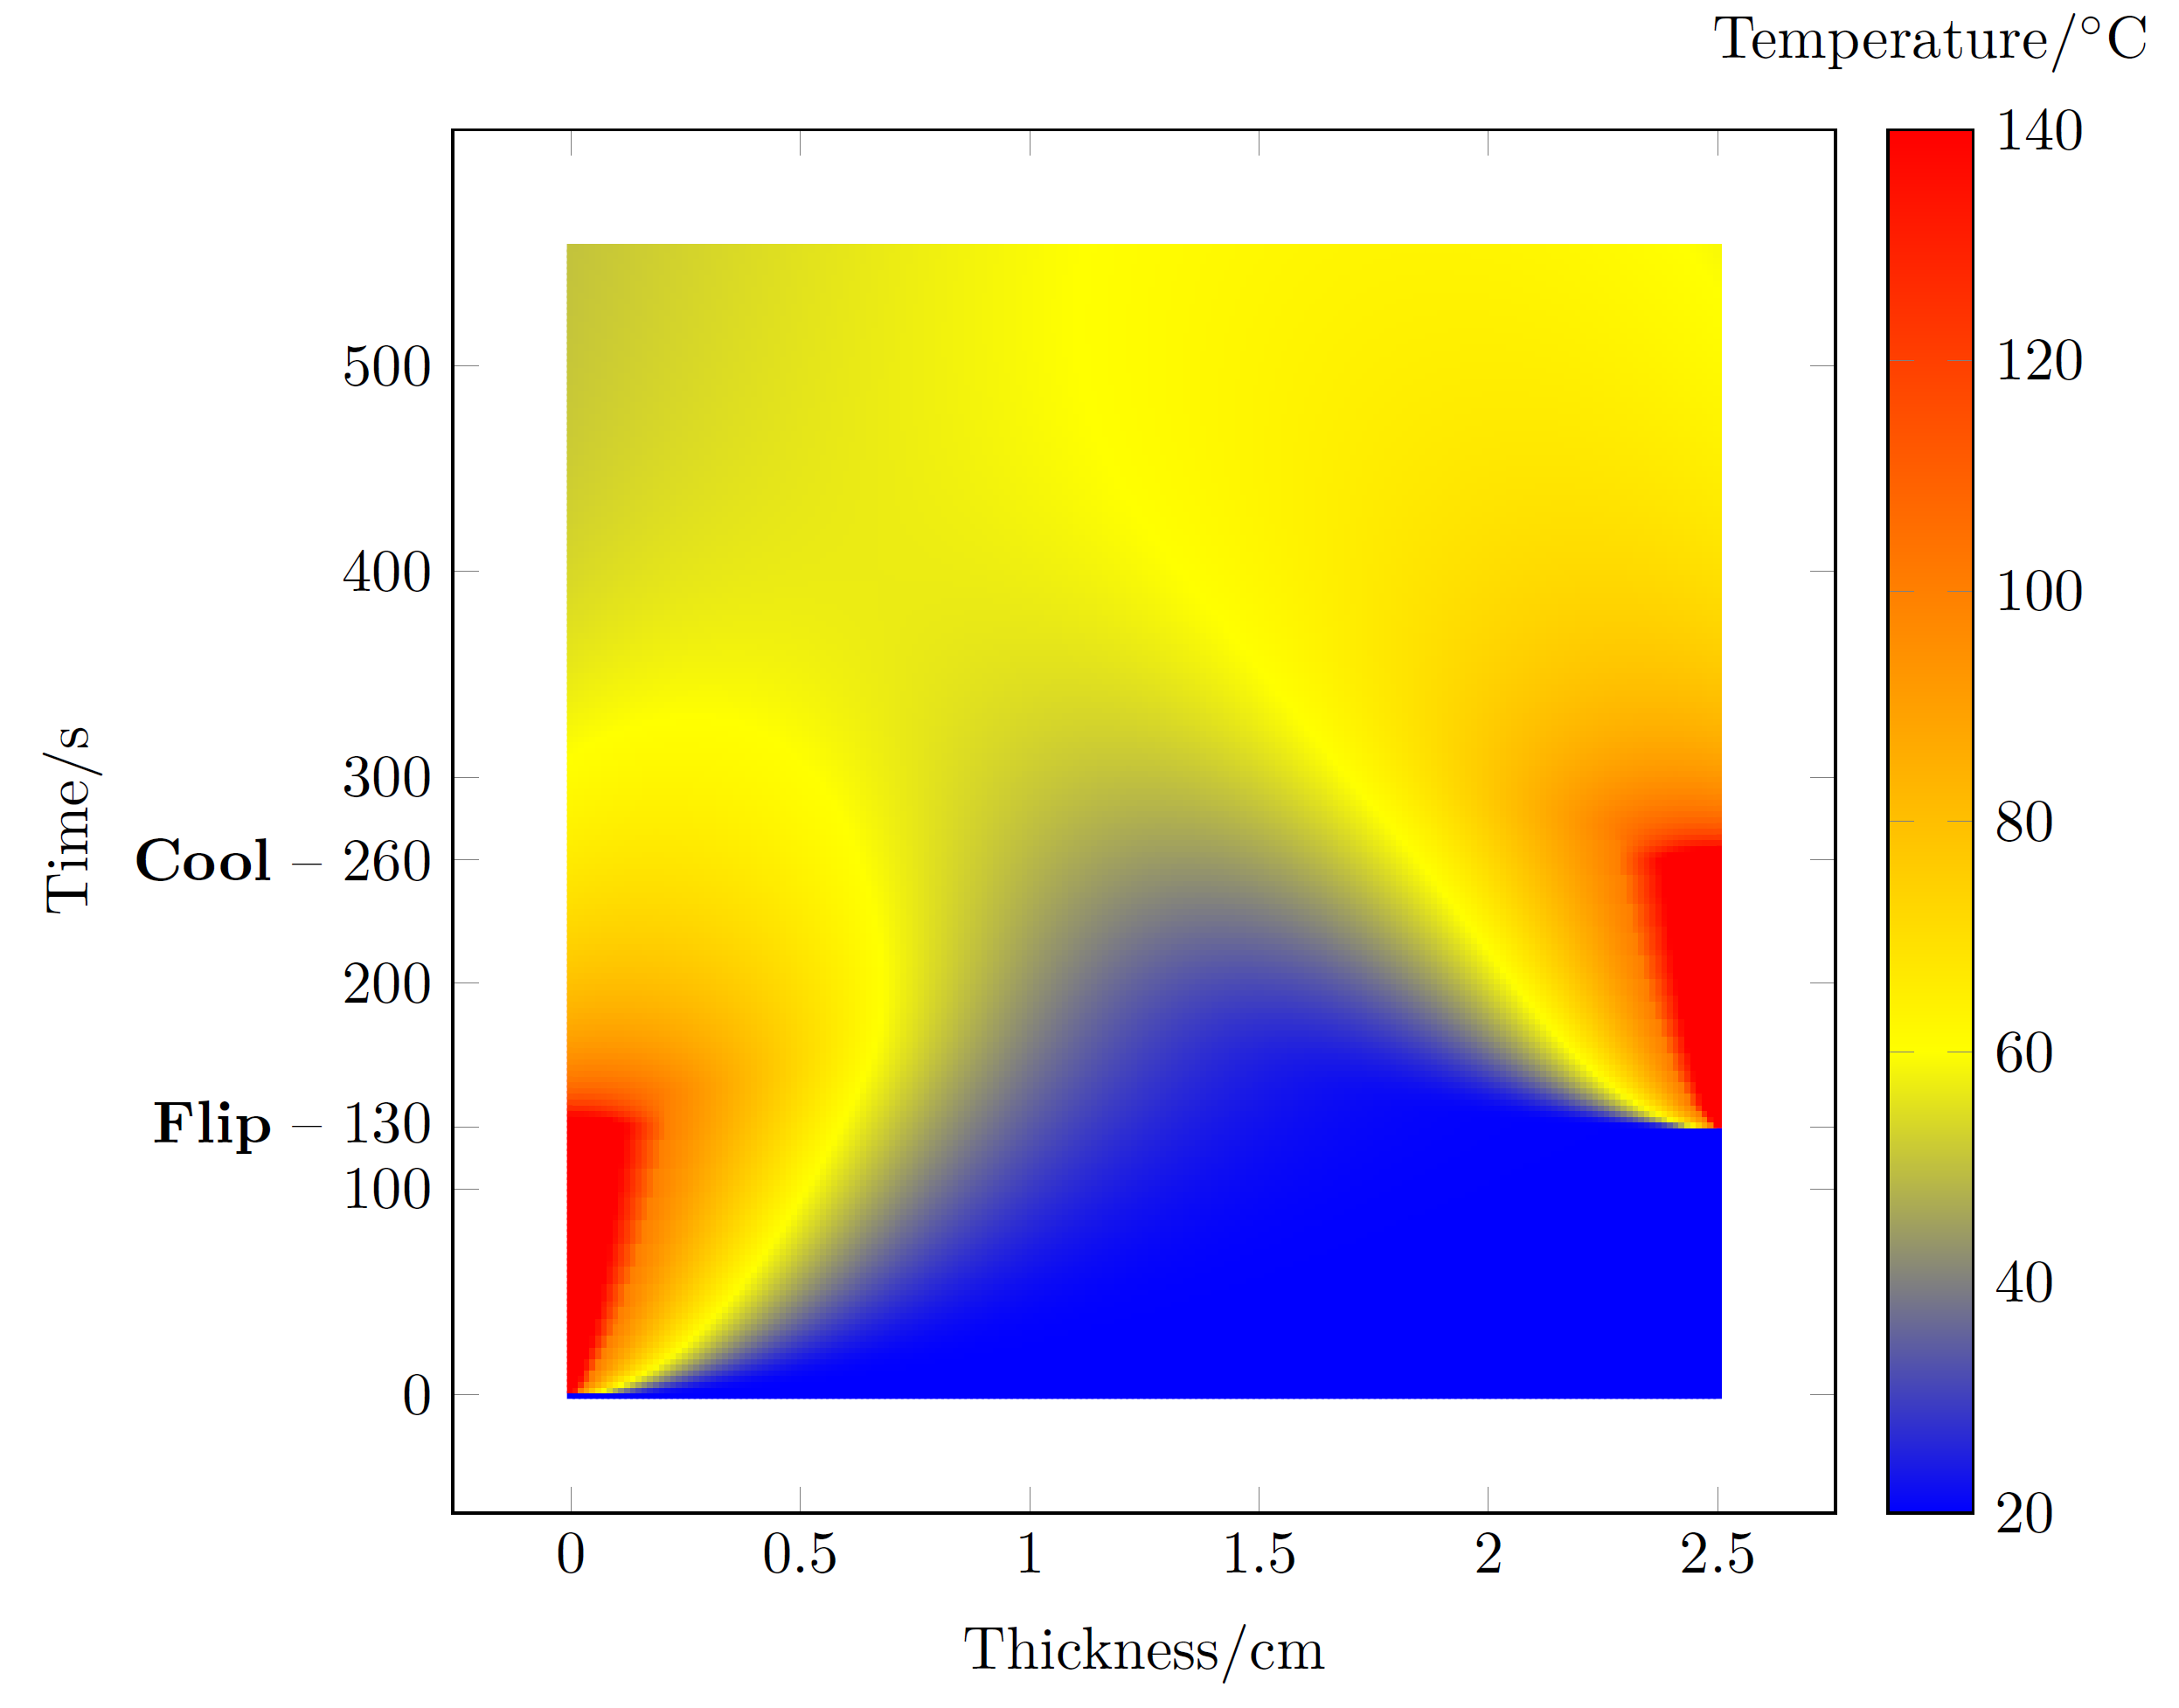
\includegraphics[width=0.6\textwidth]{./img/single-flip-heatmap.png}
		\caption{A heat map showing how the temperature along the thickness of the steak changes with time, for the single-flip sear cooking method. The steak is flipped (as marked) at $t=130\;\mathrm{s}$, and removed from the heat to cool at $t=260\;\mathrm{s}$. The higher temperatures are clipped to 140 $^\circ\text{C}$ for better definition of the important temperature ranges.}
		\label{fig:single-flip-heatmap}
	\end{figure}
	
	\begin{figure}[H]
		\centering
		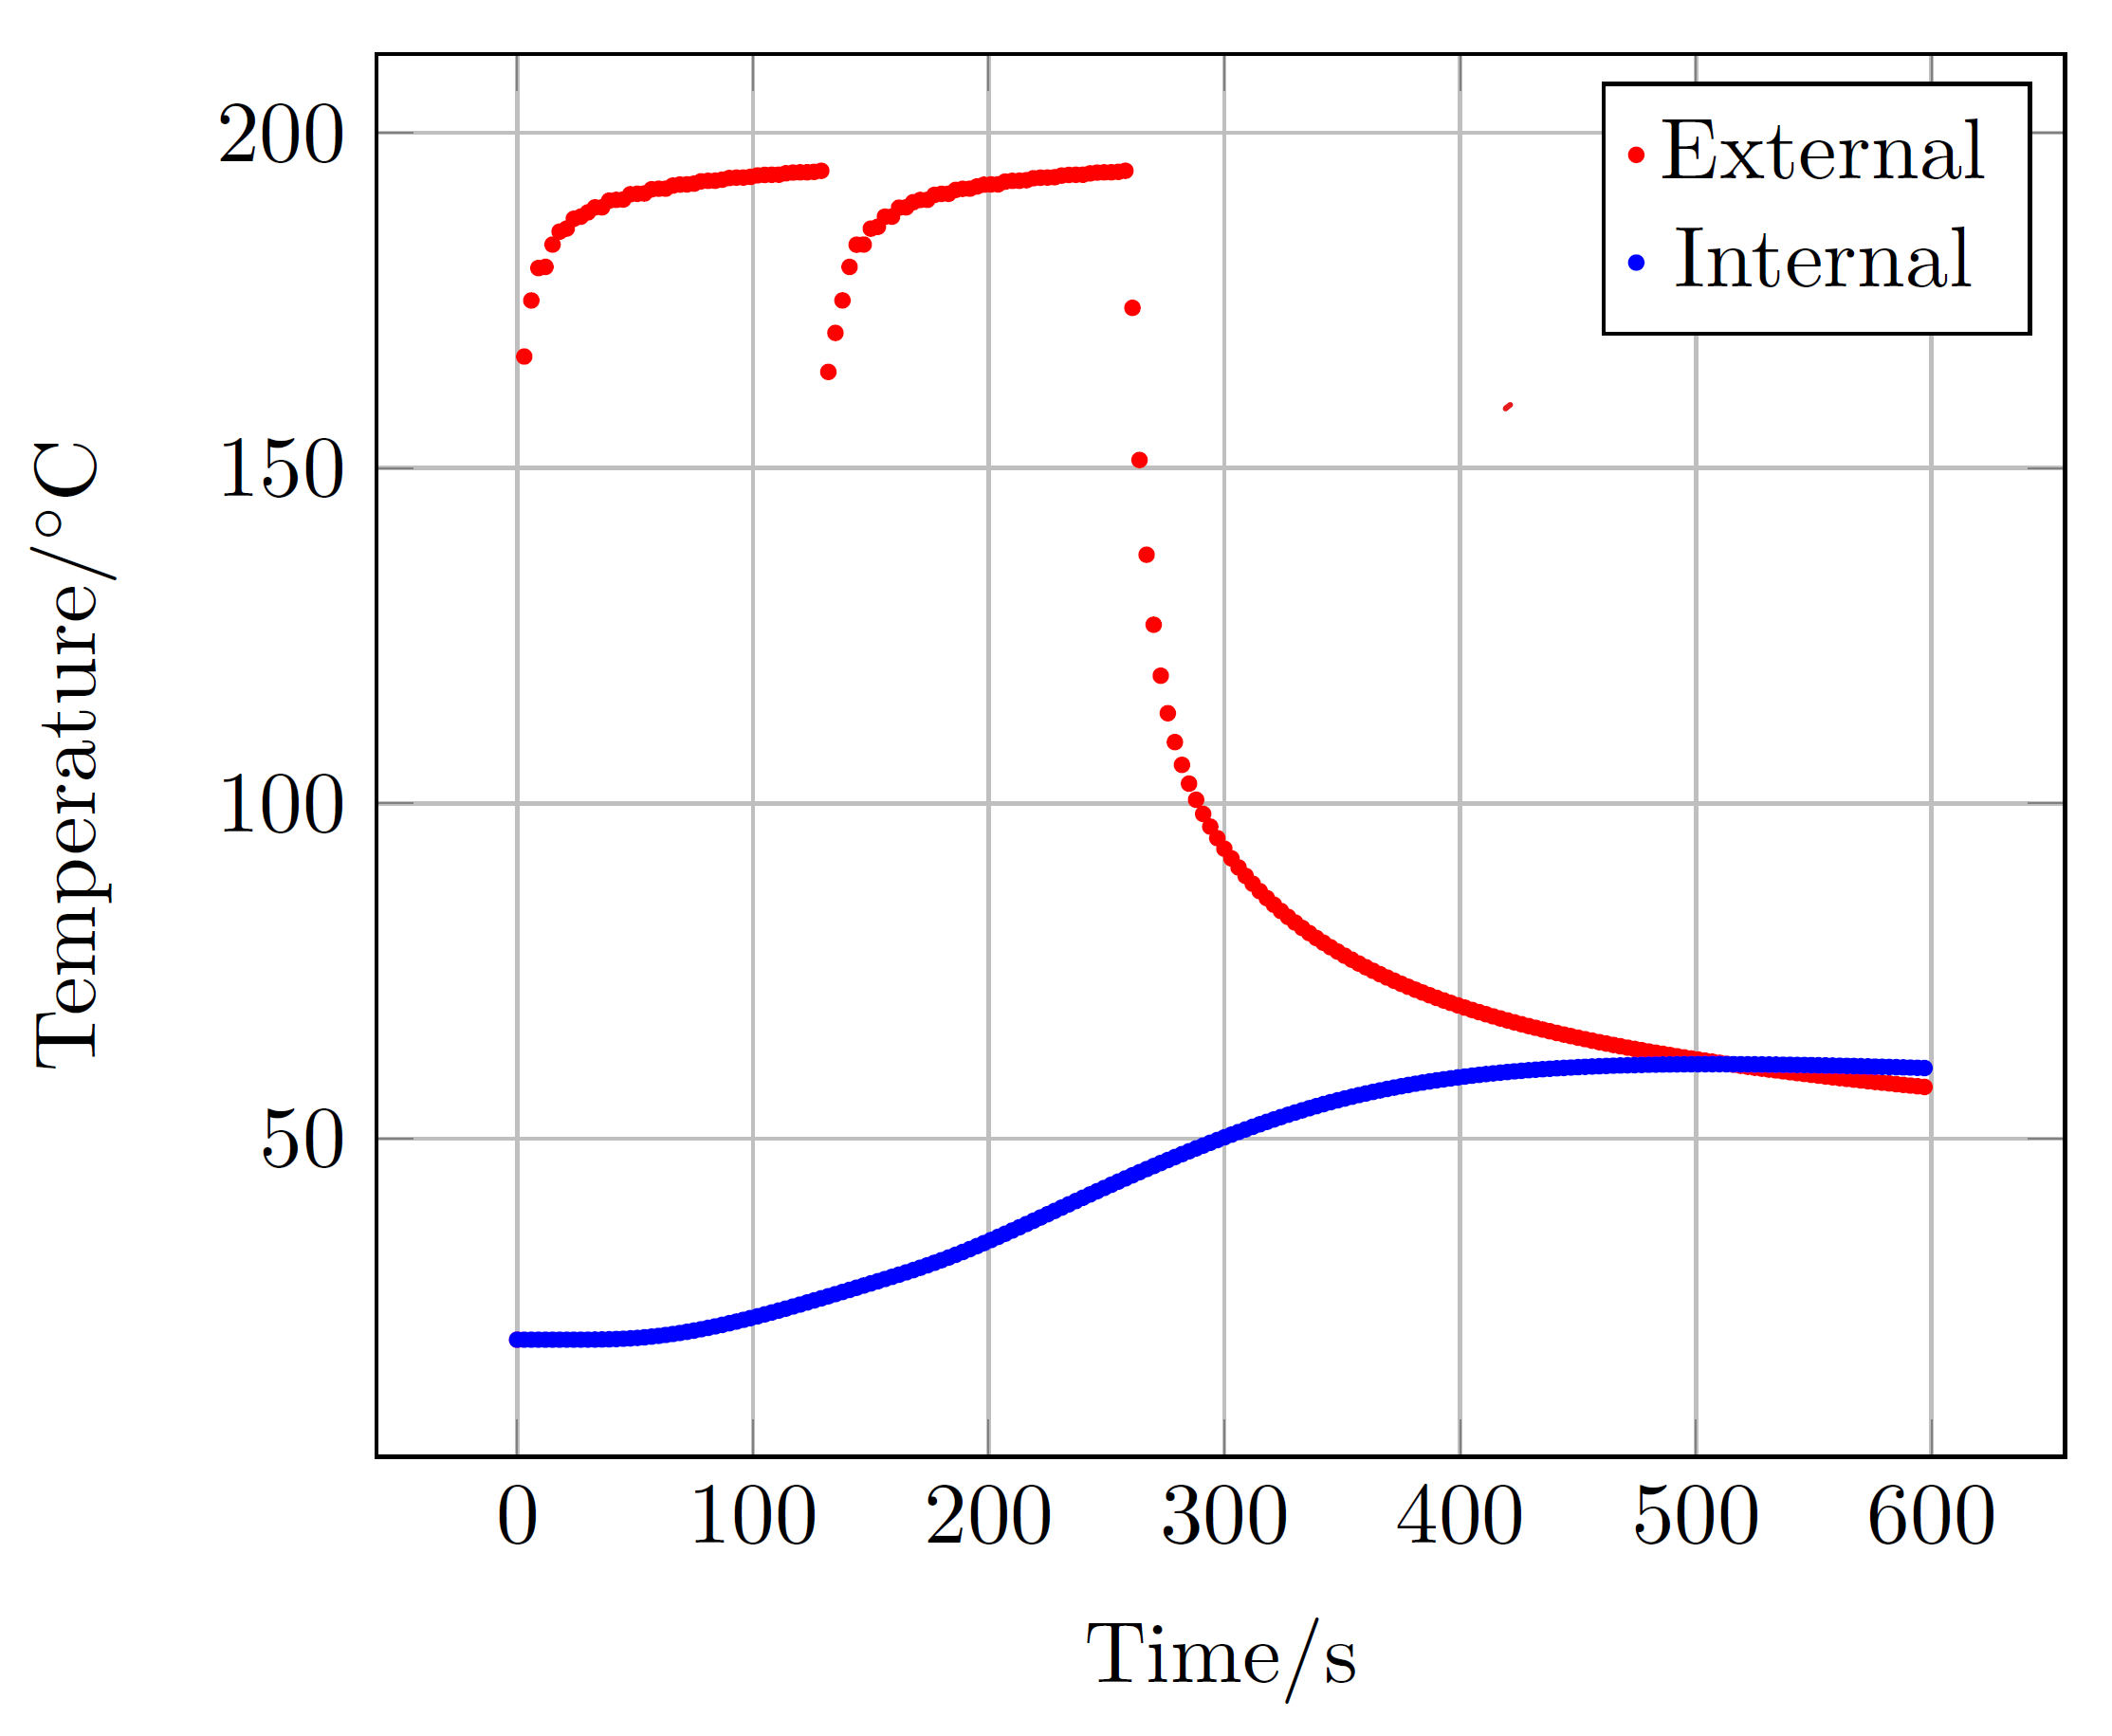
\includegraphics[width=0.5\textwidth]{./img/temps-single-sear.png}
		\caption{A graph showing how the internal (blue points) and maximum external (red points) temperatures change over time, for the single-flip sear cooking method.}
		\label{fig:single-flip-temps}
	\end{figure}
	
	When neglecting the carry-over cooking time, my modelling matches reasonably well with experimental results\cite{steak_modelling}. With an internal temperature of $50\; ^\circ$ being reached in 300 s in my model vs. the experimental 400 s. I believe my model also overestimates the carry-over cooking, usually estimated at up to $5\; ^\circ$ for a steak\cite{carryover}. While the values obtained from my model are out from the experimental ones, they still give a good estimate for the temperatures reached during cooking.
	
	\subsection{Rapid-flip pan sear}
	
	The next cooking method is very similar to the previous searing method, and has the same combinations of boundary conditions, however it is flipped every 15 seconds -- a total of 9 times. A heat map for this method is shown in \autoref{fig:rapid-flip-heatmap}. Two things are immediately obvious from this: the cooking time is significantly shorter than the single-flip method; and the cook is a lot less skewed. These are both due to each side of the steak spending less continuous time exposed to the air.
	
	\begin{figure}[H]
		\centering
		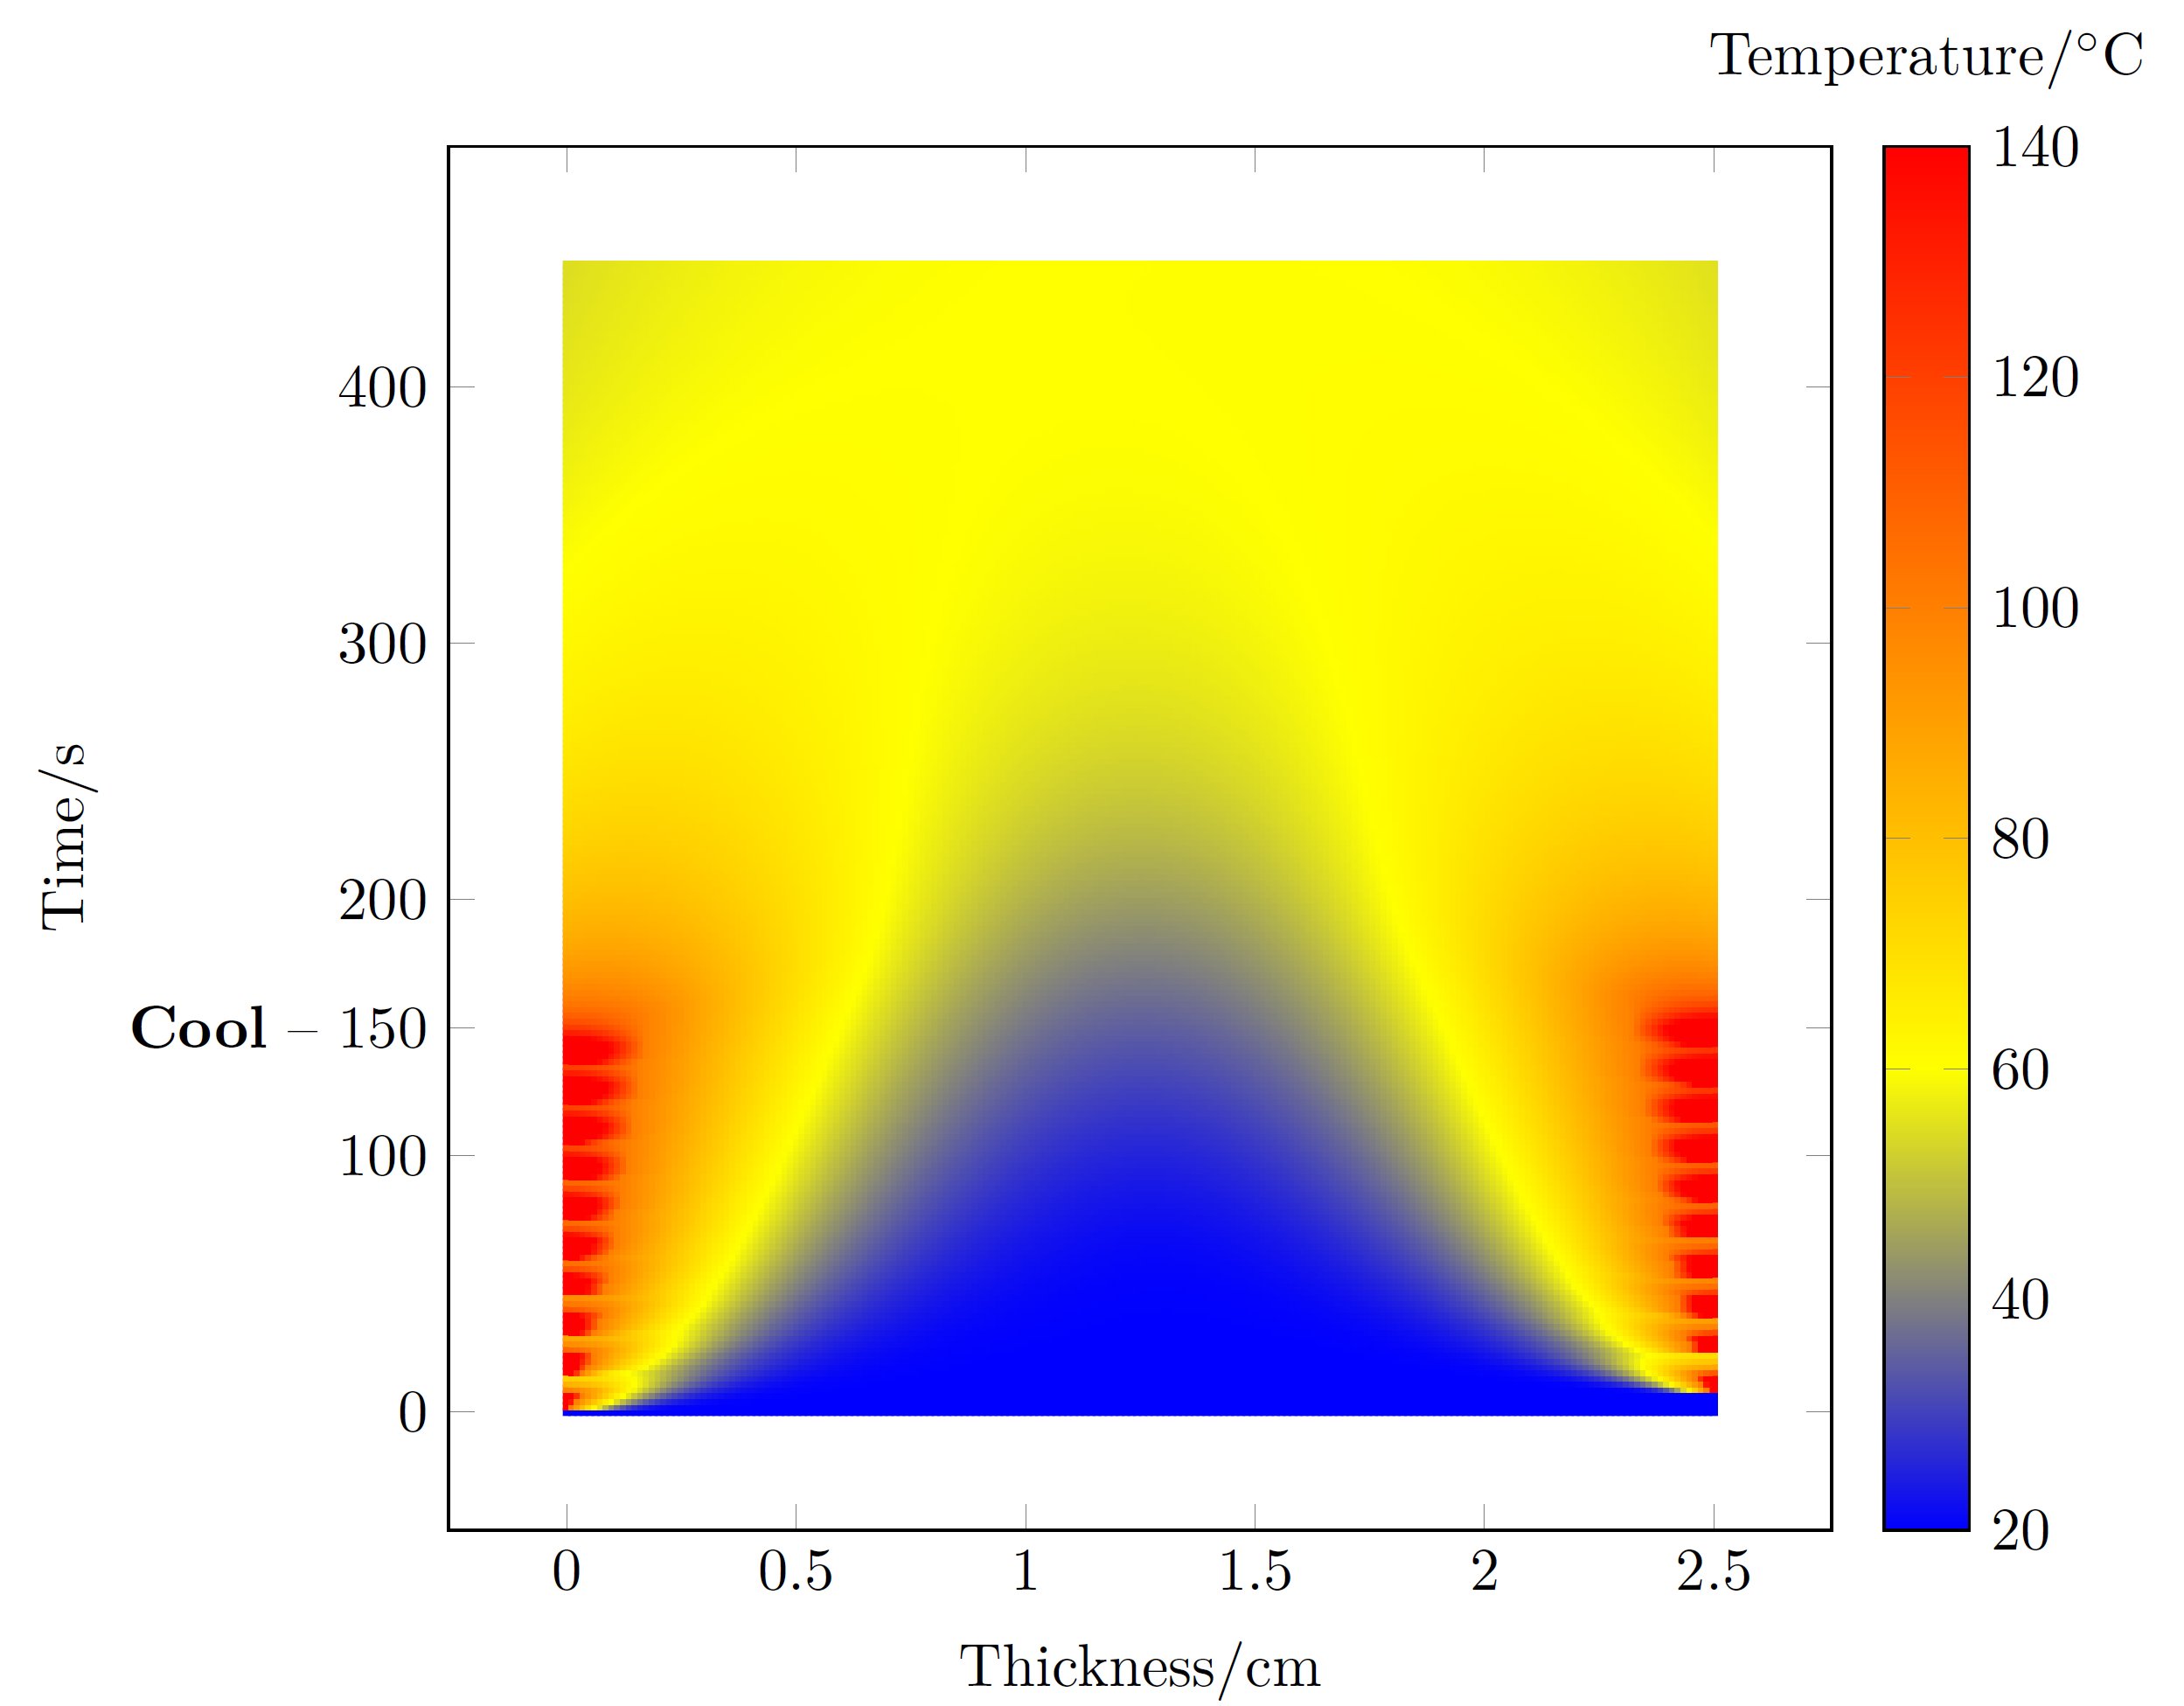
\includegraphics[width=0.6\textwidth]{./img/rapid-flip-heatmap.png}
		\caption{A heat map showing how the temperature along the thickness of the steak changes with time for the rapid-flip searing method. The steak is flipped every 15 seconds, and begins its cooling period at $t=150\;\mathrm{s}$. The higher temperatures are clipped to 140 $^\circ\text{C}$ for better definition of the important temperature ranges.}
		\label{fig:rapid-flip-heatmap}
	\end{figure}
	
	\begin{figure}[H]
		\centering
		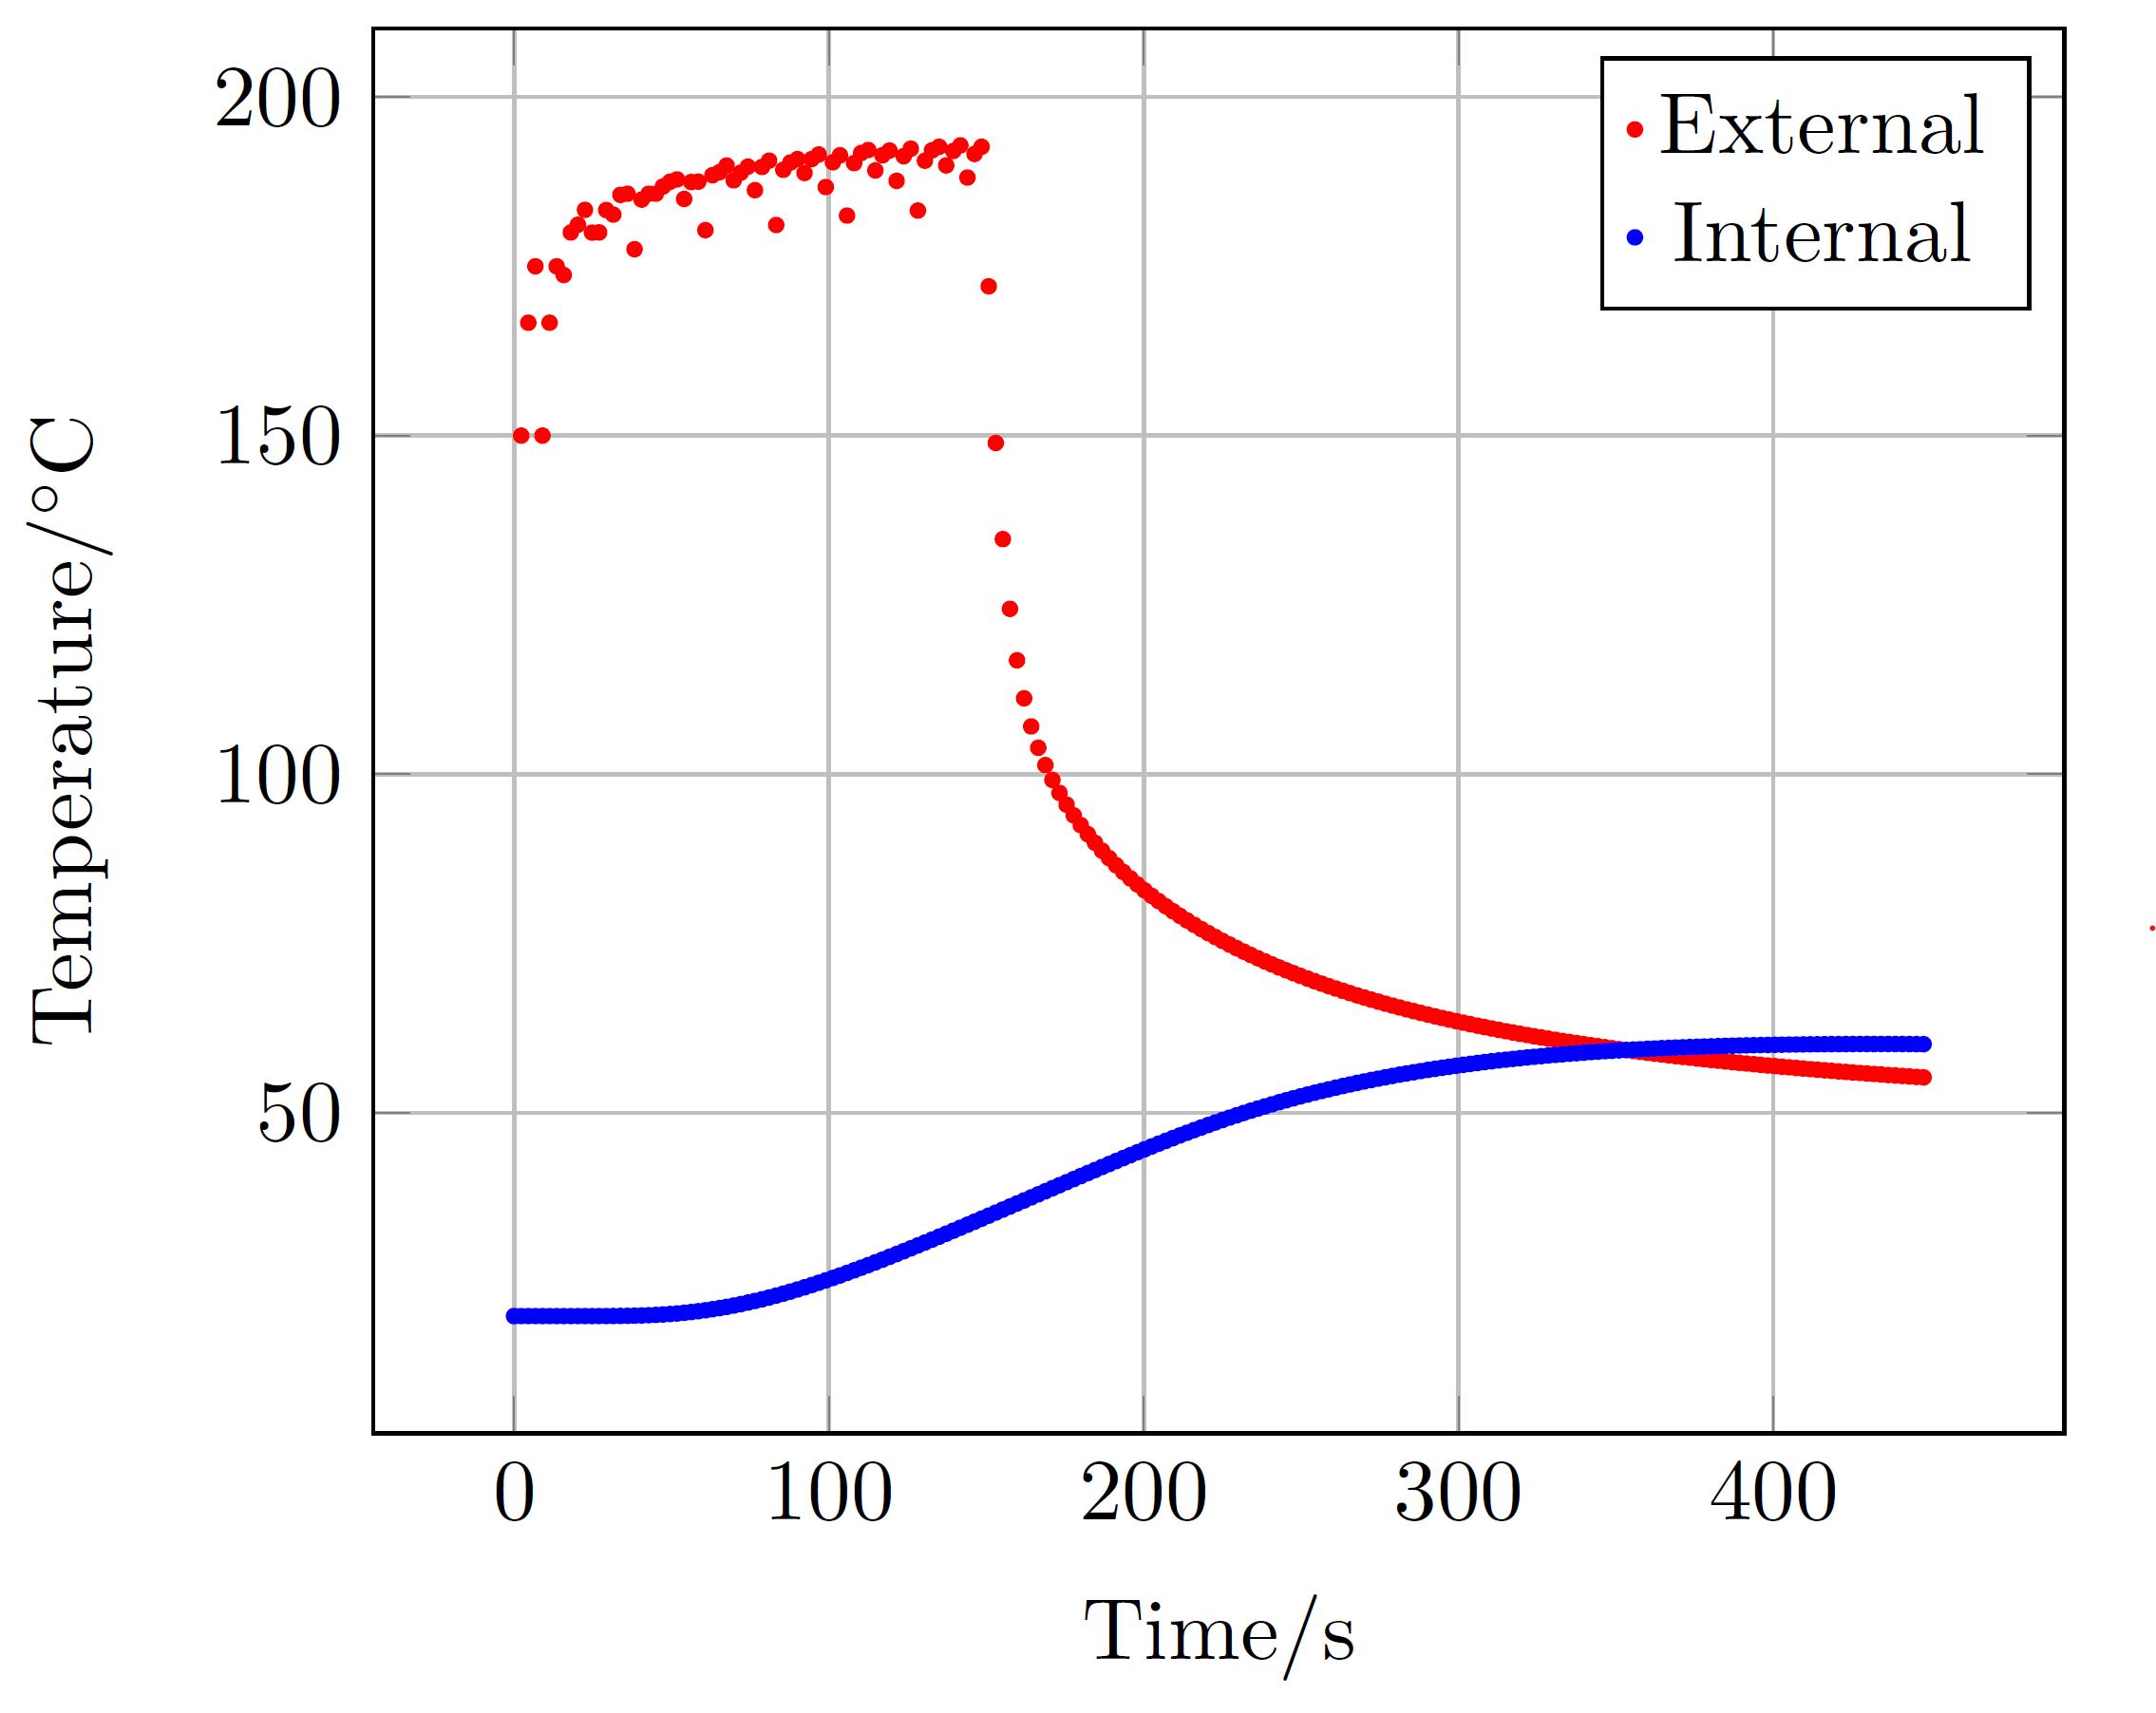
\includegraphics[width=0.5\textwidth]{./img/temps-rapid-sear.png}
		\caption{A graph showing how the internal (blue points) and maximum external (red points) temperatures change over time, for the rapid-flip sear cooking method.}
		\label{fig:rapid-flip-temps}
	\end{figure}
	
	\subsection{Medium-temperature reverse sear}
	
	This next method is one of two reverse searing methods. Where $\tau_O$ is the time spent in the oven, the boundary conditions for this general method are:
	\begin{enumerate}
		\item For $0 \leq t \leq \tau_O$: both the $x=0$ and $x=w$ boundary conditions are a steak-air boundary condition with the air at $T=T_O$, some oven temperature.
		\item For $\tau_O < t \leq \tau_O + \tau_S$: the first set of boundary conditions of the single-flip sear apply, but with $x=0$ held at a higher $T= 270\;^\circ\mathrm{C}$.
		\item For $\tau_O + \tau_S < t \leq \tau_O + 2\tau_S$: the boundary conditions are flipped.
		\item Finally, for $t > \tau_O + 2\tau_S$: the boundary conditions at $x=0$, and $x=w$ are a room-temperature air boundary condition.
	\end{enumerate}
	
	In this first case, $T_O = 180\;^\circ\mathrm{C}$, $\tau_S = 30\;\mathrm{s}$, and $\tau_O = 530\;\mathrm{s}$. A heat map for this cooking method is shown in \autoref{fig:medium-temp-reverse-sear}.
	
	\begin{figure}[H]
		\centering
		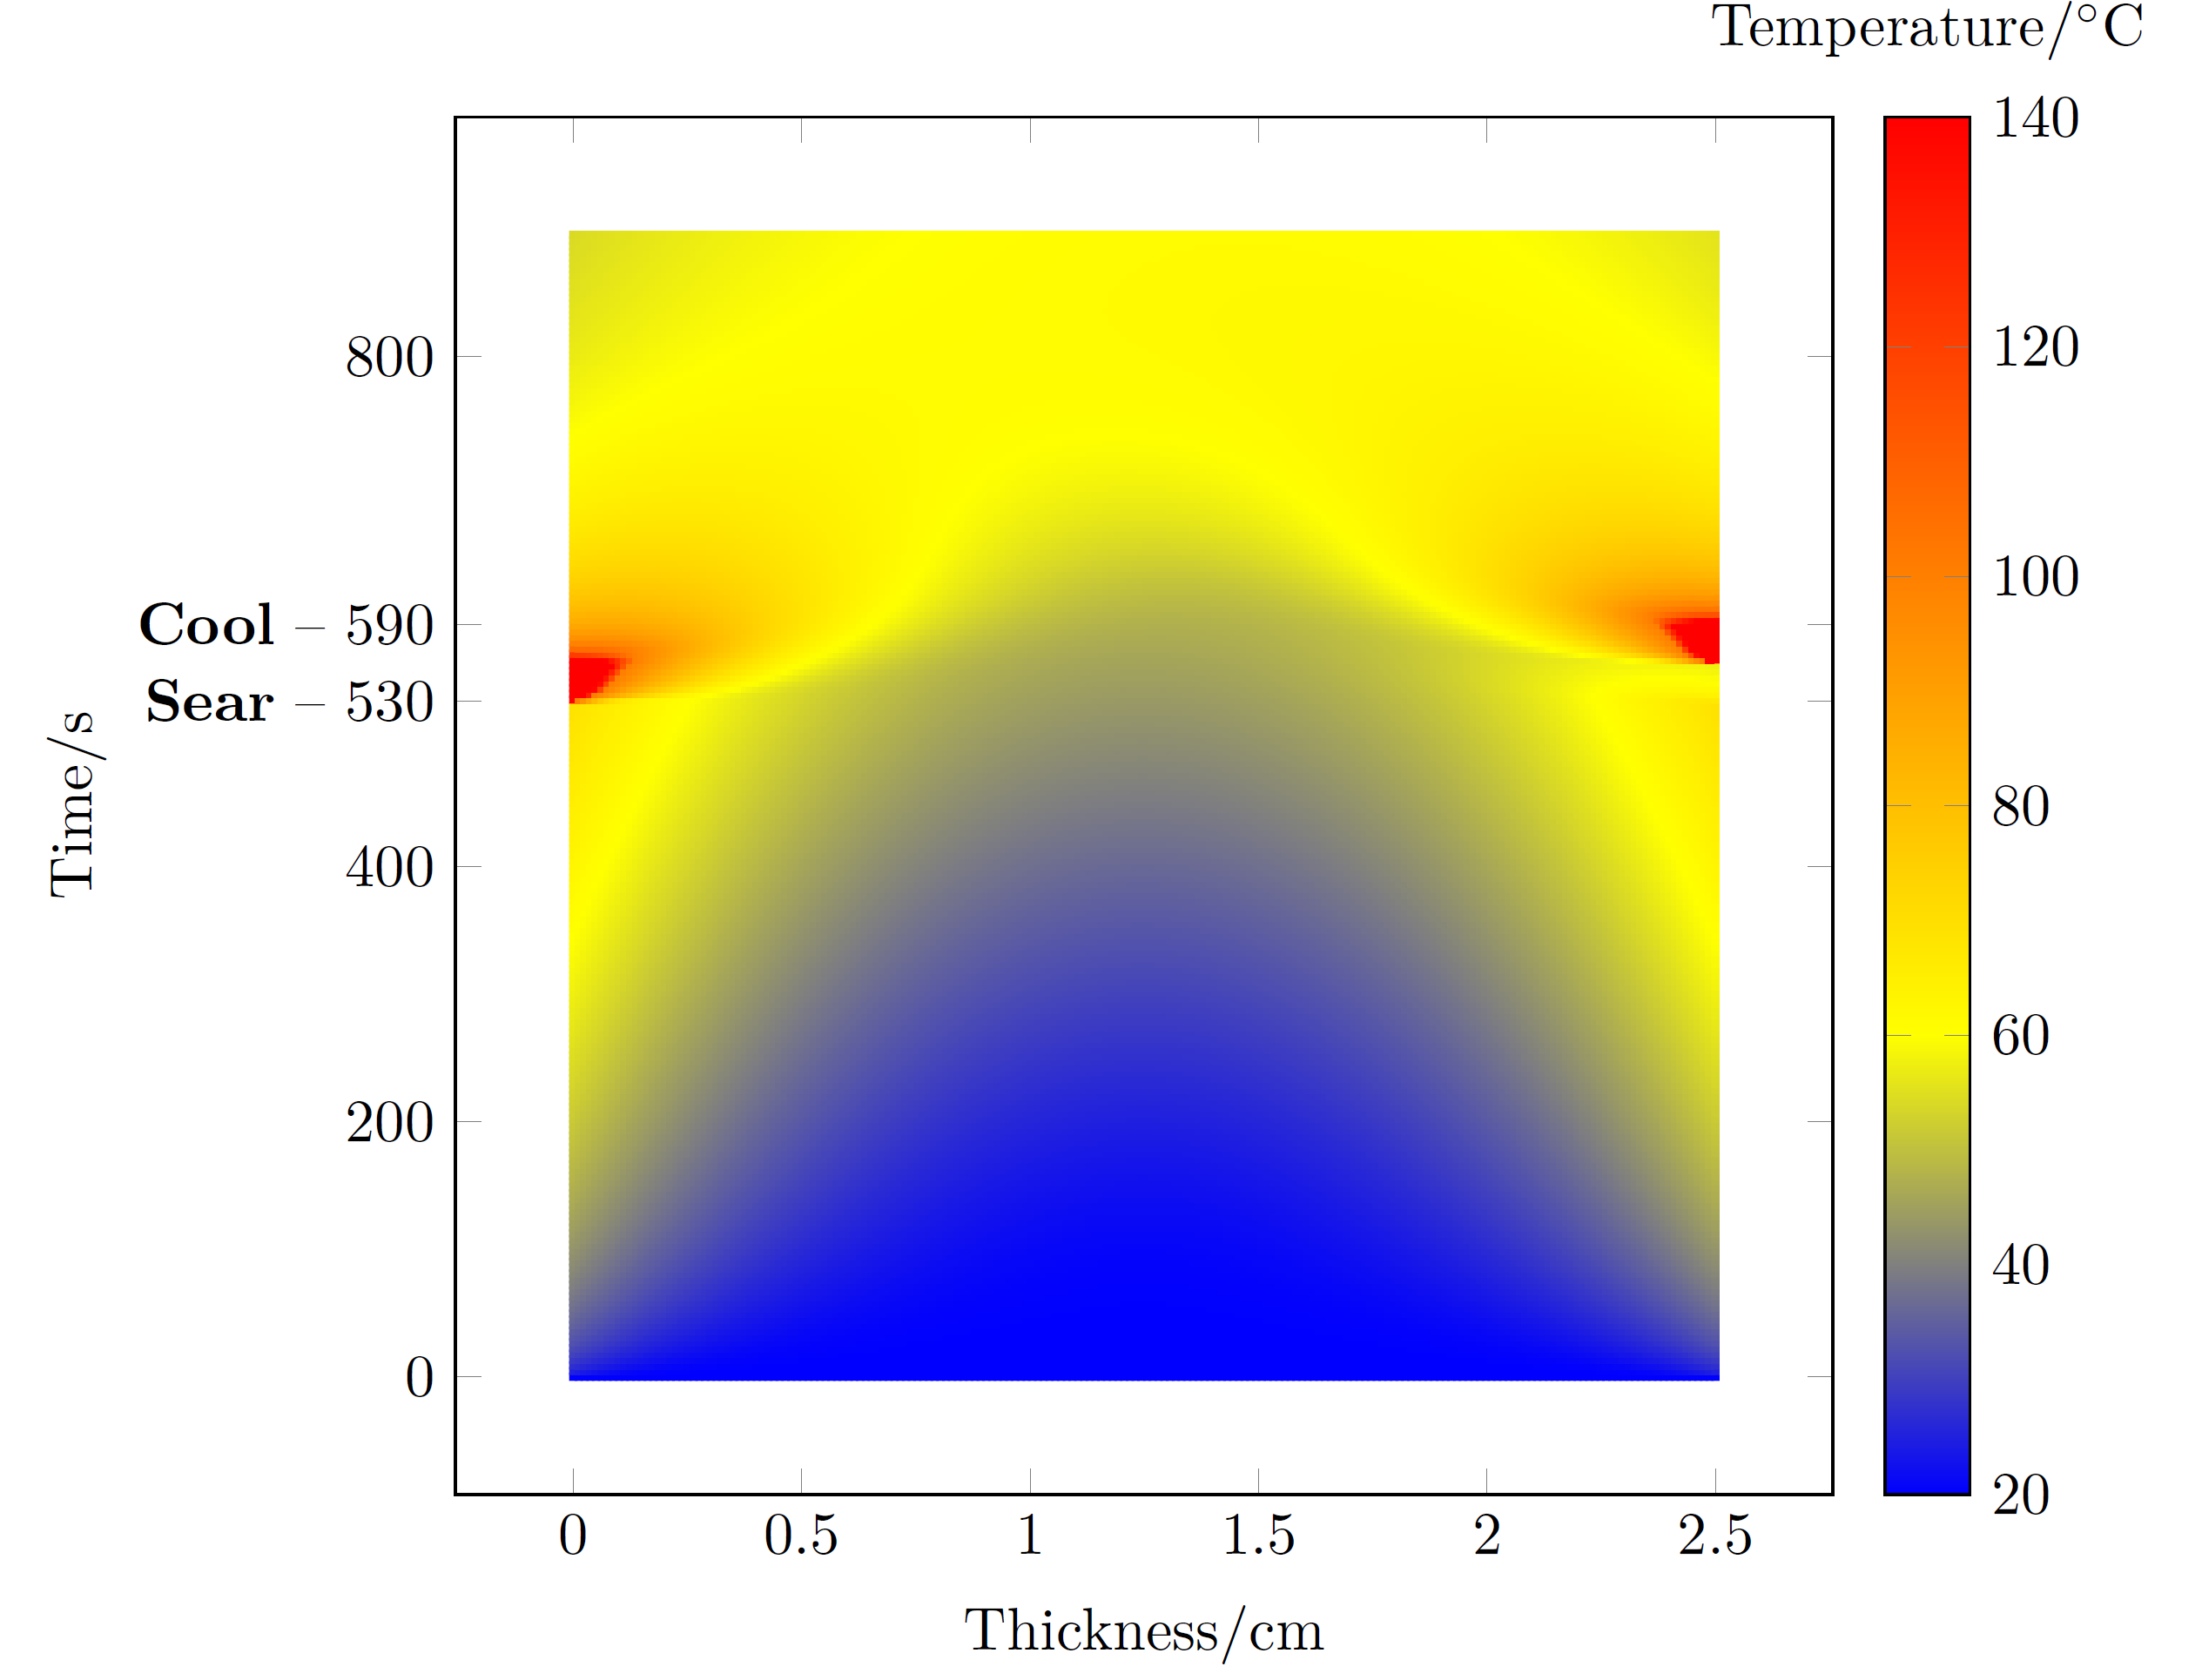
\includegraphics[width=0.6\textwidth]{./img/med-temp-reverse-sear.png}
		\caption{A heat map showing how the temperature along the thickness of the steak changes with time for the medium-temperature reverse searing method. The steak is heated in a 180 $^\circ\text{C}$ oven first, followed by a pan sear at 270 $^\circ \text{C}$ for $530 \leq t \leq 590\;\mathrm{s}$. The higher temperatures are clipped to 140 $^\circ\text{C}$ for better definition of the important temperature ranges.}
		\label{fig:medium-temp-reverse-sear}
	\end{figure}
	
	\begin{figure}[H]
		\centering
		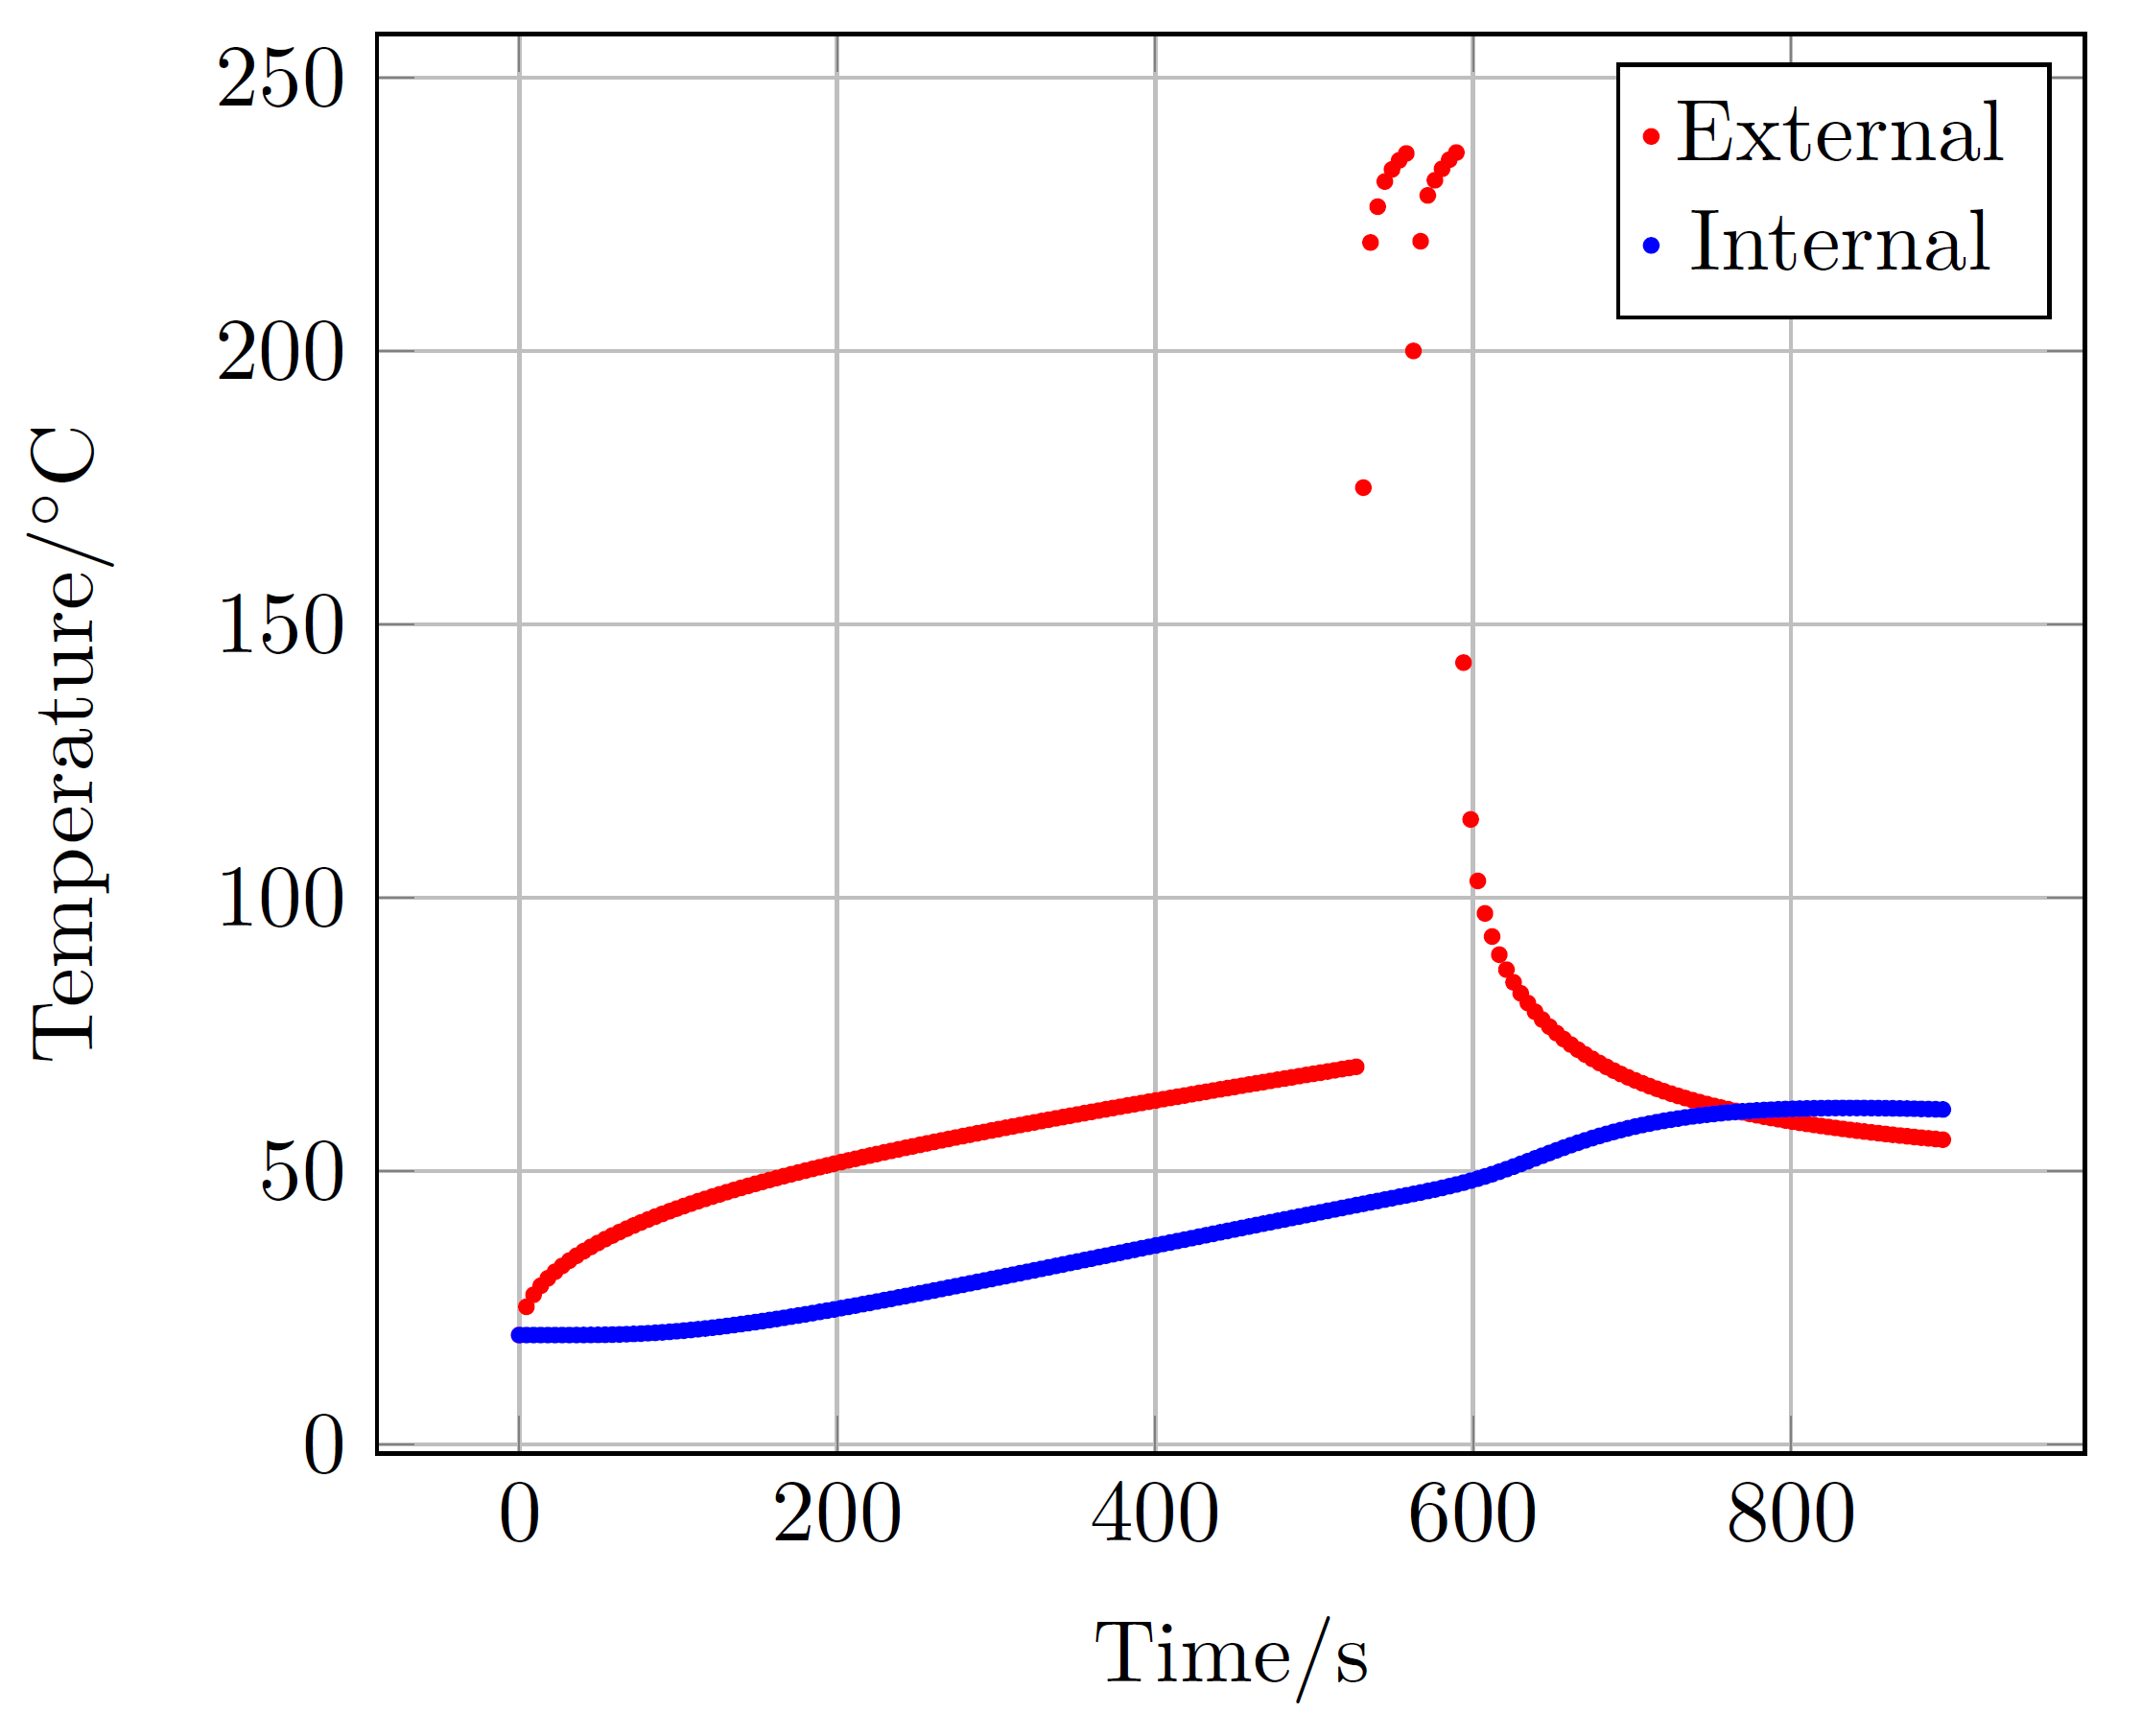
\includegraphics[width=0.5\textwidth]{./img/temps-med-reverse.png}
		\caption{A graph showing how the internal (blue points) and maximum external (red points) temperatures change over time, for the medium-temperature reverse sear cooking method.}
		\label{fig:med-reverse-sear-temps}
	\end{figure}
	
	\subsection{Low-temperature reverse sear}
	
	The final method is identical to the previous one, but with an oven temperature $T_O = 100\;^\circ\text{C}$. A heat map for this cooking method is shown in \autoref{fig:low-temp-reverse-sear}.
	
	\begin{figure}[H]
		\centering
		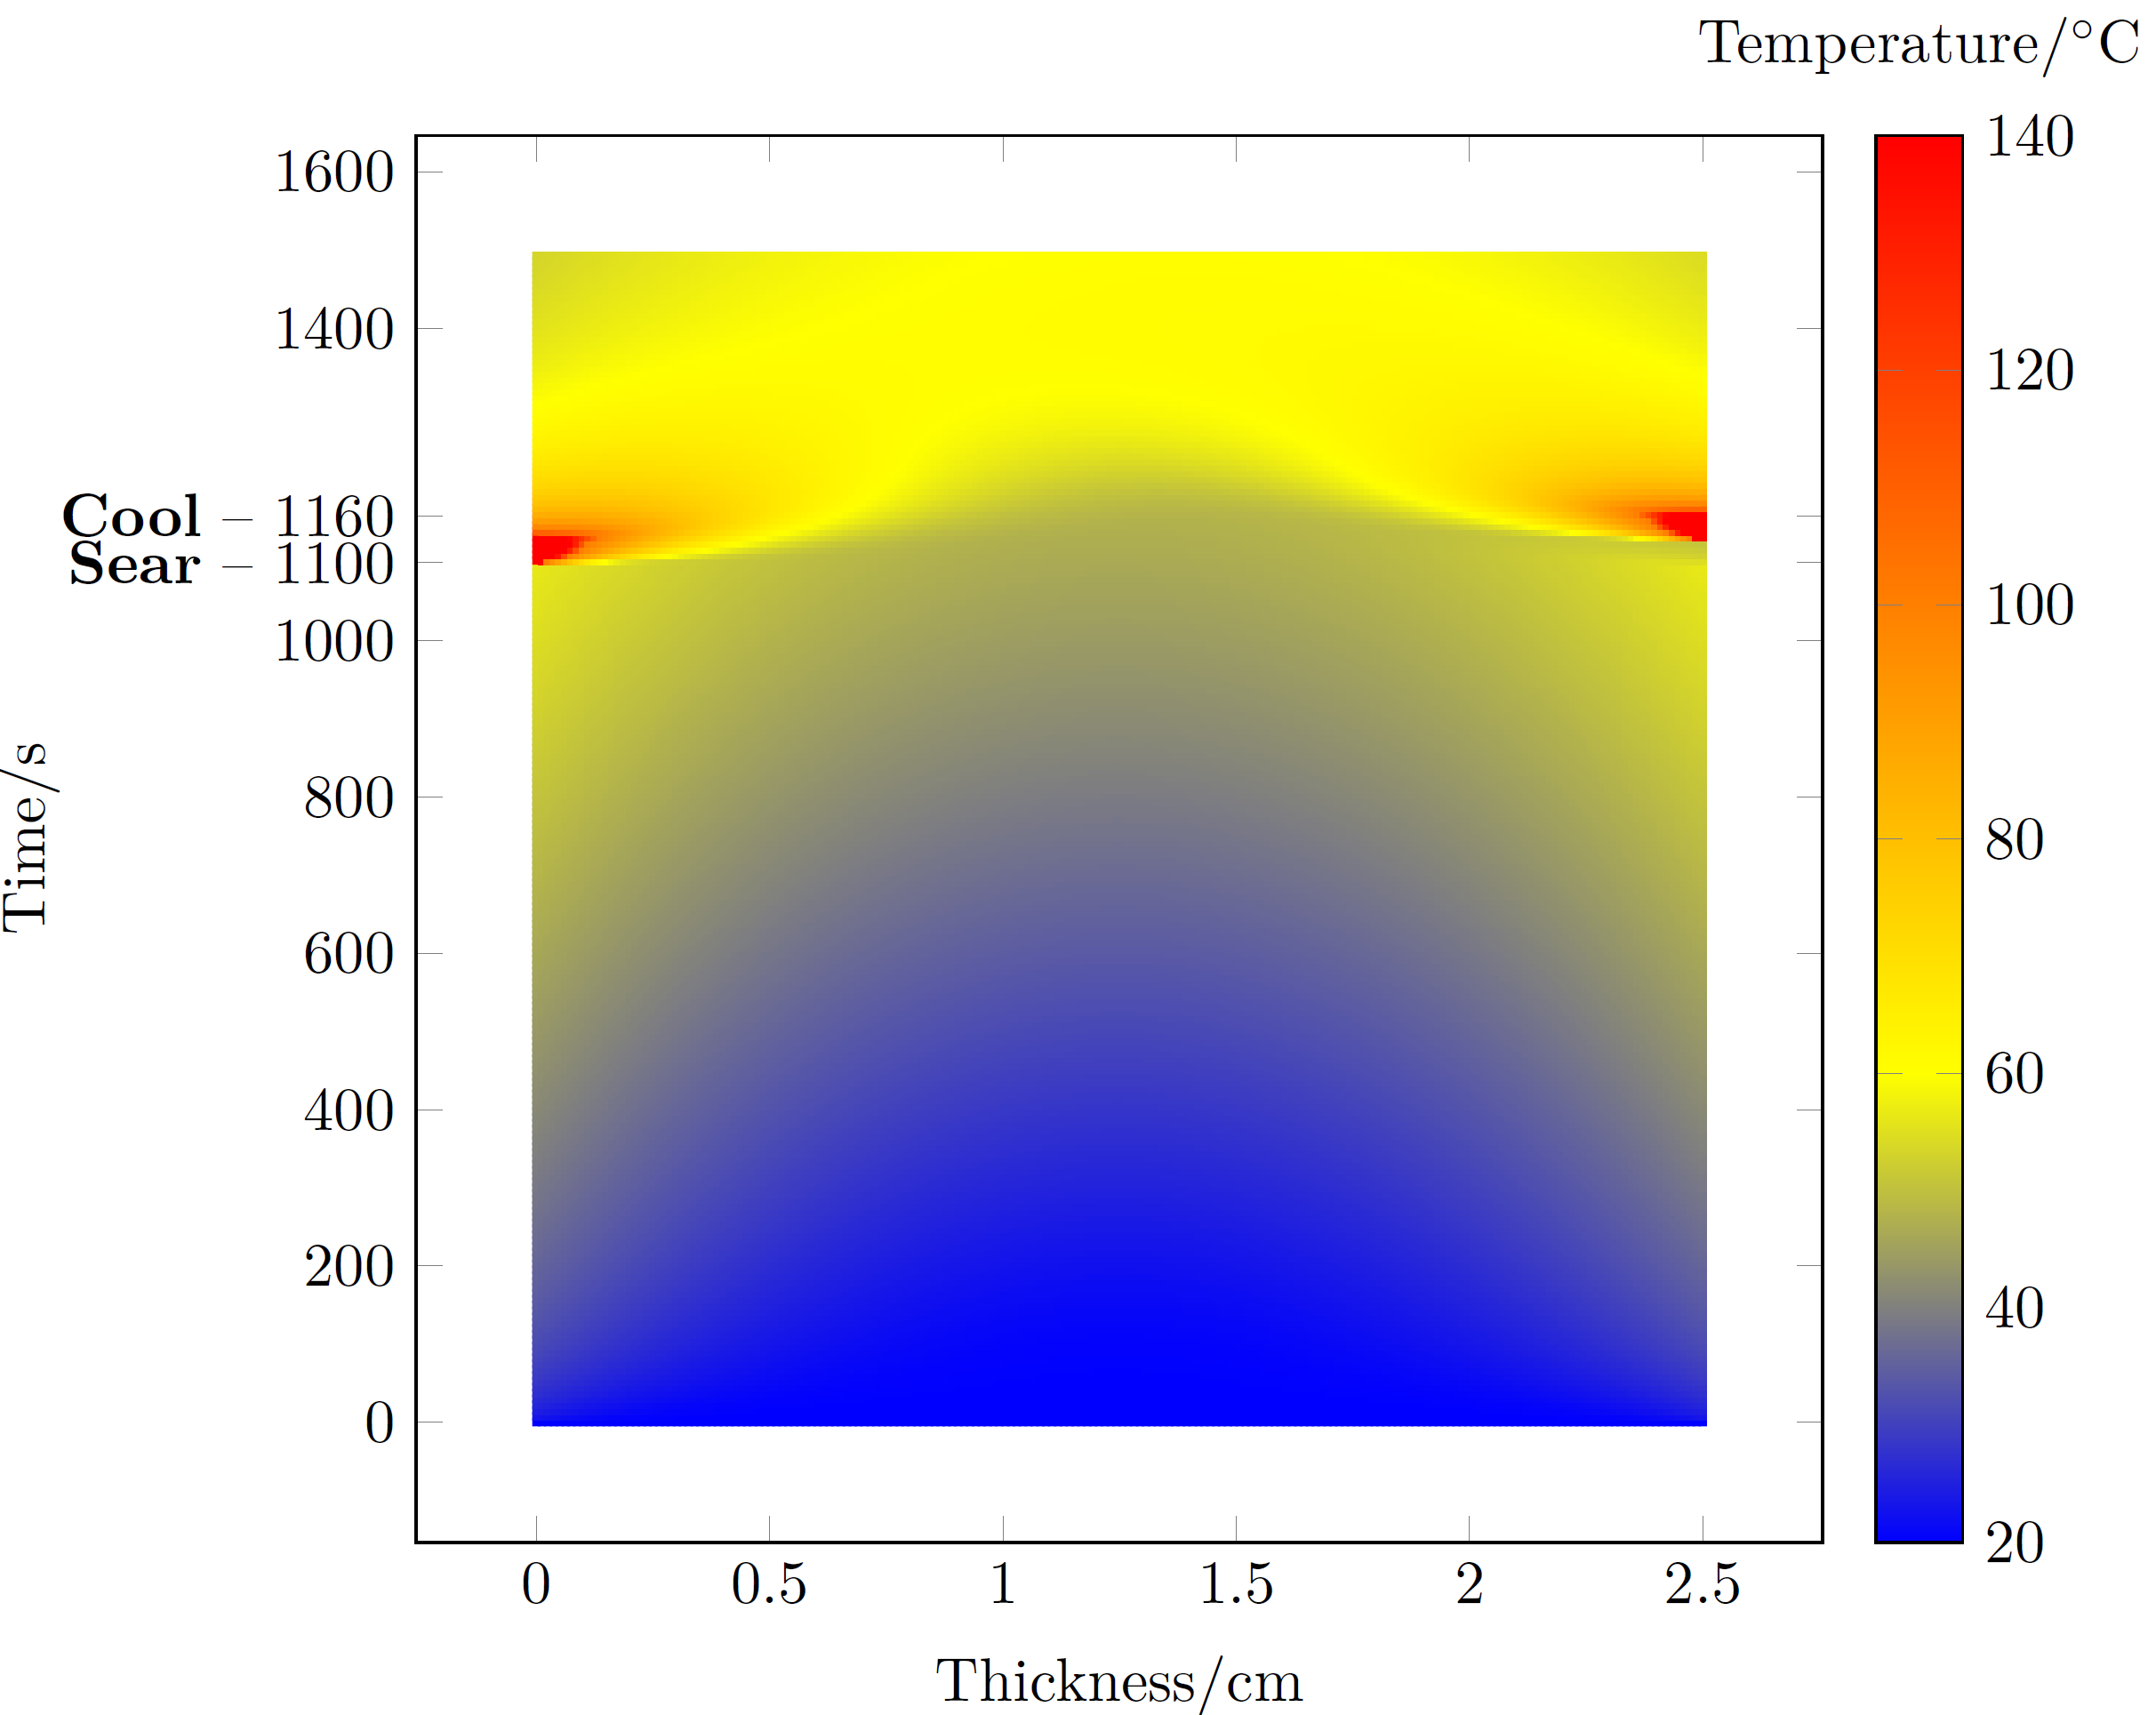
\includegraphics[width=0.6\textwidth]{./img/low-temp-reverse-sear.png}
		\caption{A heat map showing how the temperature along the thickness of the steak changes with time for the medium-temperature reverse searing method. The steak is heated in a 100 $^\circ\text{C}$ oven first, followed by a pan sear at 270 $^\circ \text{C}$ for $1100 \leq t \leq 1160\;\mathrm{s}$. The higher temperatures are clipped to 140 $^\circ\text{C}$ for better definition of the important temperature ranges.}
		\label{fig:low-temp-reverse-sear}
	\end{figure}
	
	\begin{figure}[H]
		\centering
		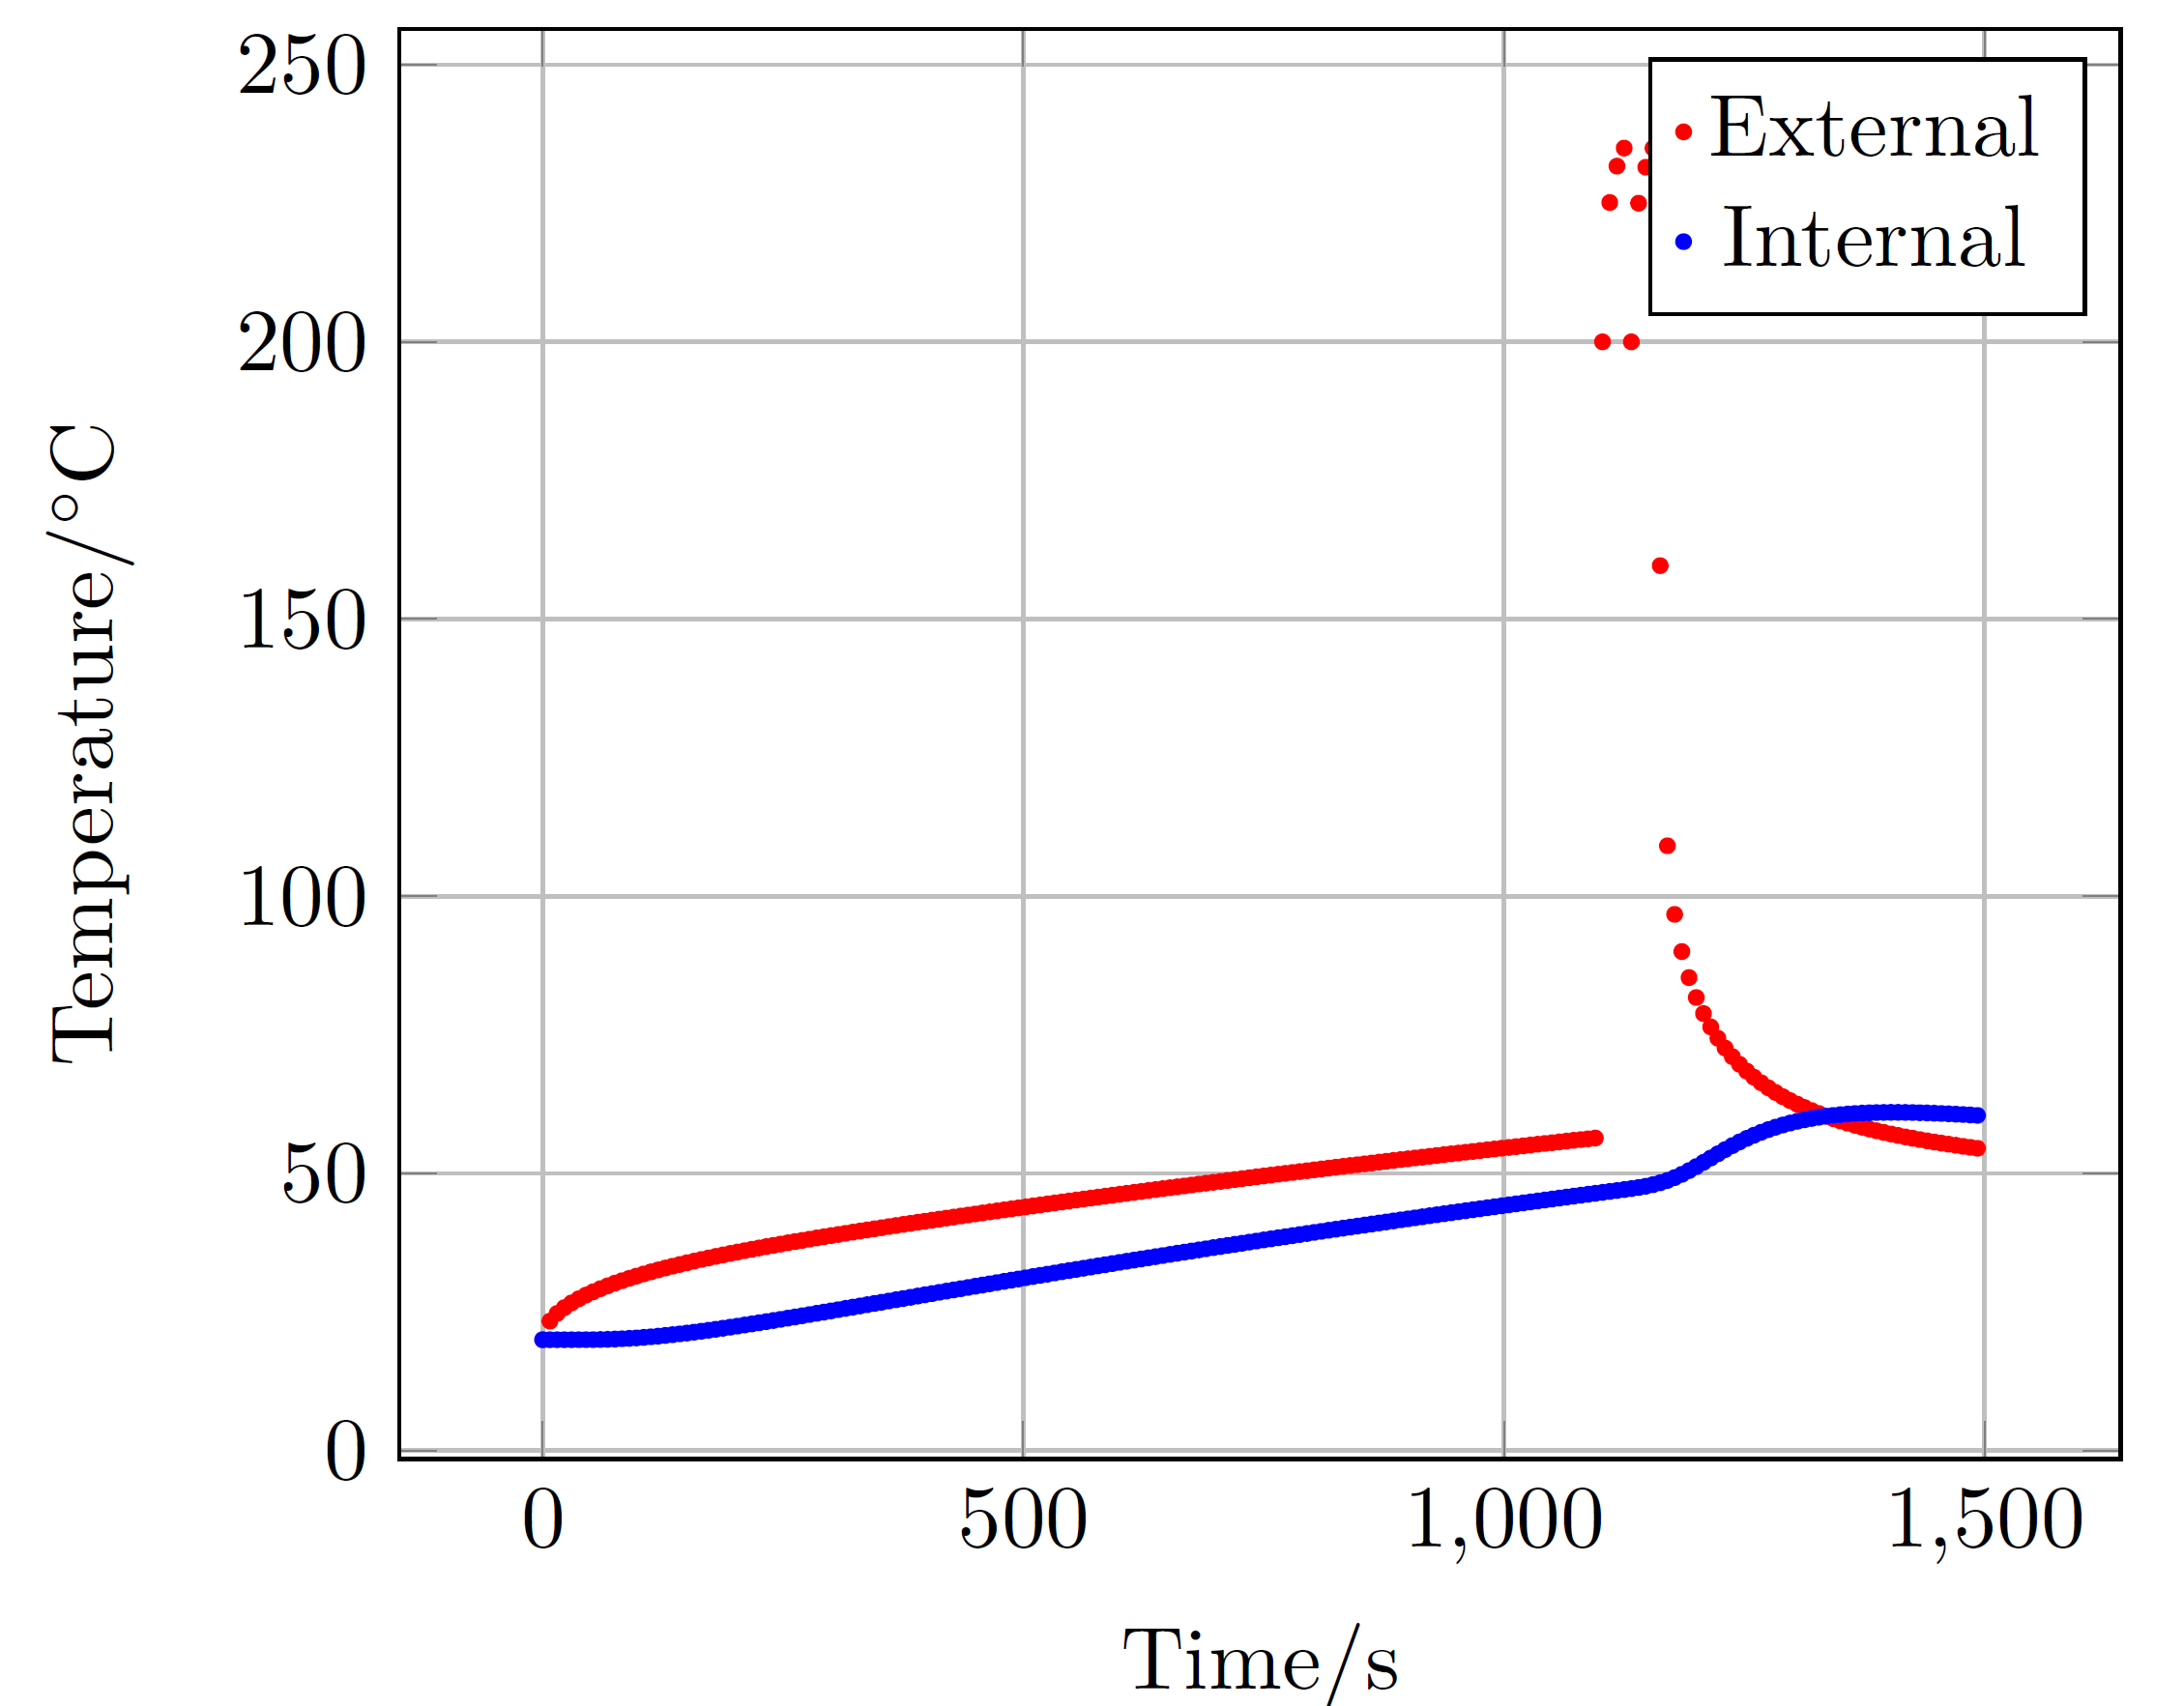
\includegraphics[width=0.5\textwidth]{./img/temps-low-reverse.png}
		\caption{A graph showing how the internal (blue points) and maximum external (red points) temperatures change over time, for the low-temperature reverse sear cooking method.}
		\label{fig:low-reverse-sear-temps}
	\end{figure}
	
	\subsection{Analysis}
	
	This simplified model of heat transfer, without a full treatment of the water/steam diffusion has still been able to give a good set of results. There is however, some divergence from what would be expected in reality. A key issue highlighted is the amount of carry-over cooking, which was $\sim 10\text{-}15\;^\circ\text{C}$ in each method. I believe this to be mainly down to the missing treatment of steam travelling through the steak redistributing the temperature, and exiting the steak carrying energy out with it. \\
	
	Nevertheless, these temperature profiles will still allow me to measure the three metrics discussed earlier, and compare each of the four cooking methods.
	
	\subsubsection{Maillard products}
	
	The values for the Maillard products metric, for each cooking method are shown in \autoref{tab:maillard_products}. The cooks with the most Maillard reaction products are clearly the reverse searing methods. Although these were seared for a much shorter time, the much hotter pan actually gives a better Maillard reaction, something that can't be done in the searing methods without overcooking (or potentially burning) the outside of the steak. Although the single flip and rapid flip methods use the same temperature pan, the rapid flip method has a shorter cooking time, but each side also spends less continuous time on the heat both contributing to its lower Maillard reaction amount.
	
	\begin{table}[H]
		\centering
		\begin{tabular}{c|c}
			\textbf{Cooking Method} & \textbf{Maillard Amount} \\
			\hline
			Single-flip sear & 125.5 \\
			Rapid-flip sear & 46.0 \\
			Medium-temperature reverse sear & 264.7 \\
			Low-temperature reverse sear & 259.6
		\end{tabular}
		\caption{A table showing the amount of Maillard reaction products for each cooking method}
		\label{tab:maillard_products}
	\end{table}
	
	\subsubsection{Evenness of cook}
	
	The values for the evenness metric, for each cooking method are shown in \autoref{tab:evenness}. The merits of rapidly flipping the steak can clearly be seen here, giving a much more even cook than the single-flip method. However, the reverse sear improves upon this further, with a lower temperature oven giving a more even cook. The gradual application of heat allows the whole steak to reach its desired internal temperature without producing a large temperature gradient. Some gradient will still be introduced when searing the steak at the end, but much less than the sear only methods.
	
	\begin{table}[H]
		\centering
		\begin{tabular}{c|c}
			\textbf{Cooking Method} & \textbf{Evenness} \\
			\hline
			Single-flip sear & $-4780$ \\
			Rapid-flip sear & $-3298$ \\
			Medium-temperature reverse sear & $-1986$ \\
			Low-temperature reverse sear & $-1696$
		\end{tabular}
		\caption{A table showing the evenness metric for each cooking method}
		\label{tab:evenness}
	\end{table}
	
	\subsubsection{Skew of cook}
	
	The values for the skew metric, for each cooking method are shown in \autoref{tab:skew}. The only cooking method with a skew that was not negligible was, as can be told from its heat map, the single-flip sear method. There is a bias towards the first side that goes on the heat, since the other side initially has no increase in temperature. There is a slight skew due to this same principle for the other cooking methods, but its effect is negligible due to the shorter searing times.
	
	\begin{table}[H]
		\centering
		\begin{tabular}{c|c}
			\textbf{Cooking Method} & \textbf{Skew}/mm \\
			\hline
			Single-flip sear & $-0.69$ \\
			Rapid-flip sear & 0.00 \\
			Medium-temperature reverse sear & 0.00 \\
			Low-temperature reverse sear & 0.00
		\end{tabular}
		\caption{A table showing the skew of each cooking method}
		\label{tab:skew}
	\end{table}
	
	\subsection{Summary}
	
	From the data gathered, it is clear that a reverse sear scores the best on all metrics, with a lower oven temperature also being better. The low-temperature, slower cook allows the centre to reach its required temperature without overcooking the regions close to the surface. The searing stage can then also be applied much more strongly as it serves only to cause the Maillard reaction, and not to cook the inside of the steak. This allows more Maillard reaction products, while also keeping searing time to a minimum, to keep the rest of the meat from overcooking.\\
	
	These advantages will become increasingly important for larger thicknesses of steak, since a single method for the application of heat cannot give the sharp temperature difference between the internal and surface temperatures. The merits of rapidly flipping a steak while searing are also clear from the results, giving a more even cook, and faster cooking time. This is while losing some amount of Maillard reaction, so the better method isn't as clear cut.
	
	\section{Conclusion}
	
	In conclusion, the best method for cooking a steak (as determined by my criteria) is a reverse searing method, with a low oven temperature. This gives the most Maillard reaction products, the most even cook, and no skew to the cook. As discussed in the introductory parts of this dissertation, many simplifications were made in the modelling used, neglecting the water transport that occurs during the cooking process, and approximating the thermal diffusion rate as temperature independent. Even with these simplifications, the results for cooking times matched well (although not as closely as the more sophisticated models\cite{steak_modelling}) with reality. \\
	
	To improve upon the modelling of heat would require a full treatment of the coupling of the diffusion and heat equations, and the inclusion of the temperature dependence of the thermophysical properties of meat. I do not believe however, that more accurate modelling would affect the evaluations made for the four different cooking methods.
	
	\pagebreak
	
	\small
	
	\bibliography{references} 
	
	\pagebreak 
	
	\section*{Appendix}
	
	As a matter of personal interest, I decided to cook three sections of the same rib-eye steak with these different methods, and then rank them in a blind trial. The three methods were: single-flip sear, rapid-flip sear, and reverse sear. The results of which are shown in \autoref{fig:steak}.
	
	\begin{figure}[H]
		\centering
		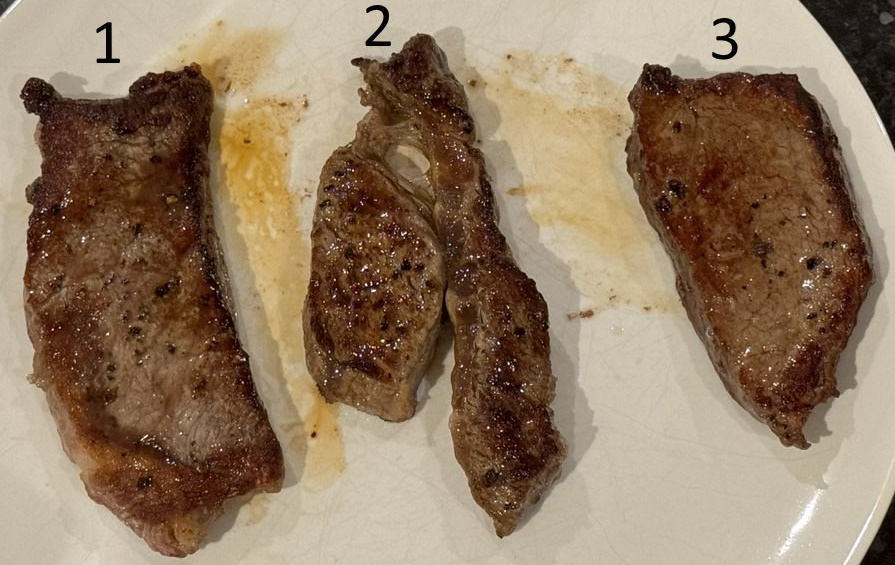
\includegraphics[width=0.9\textwidth]{./img/steak-top.jpeg}
		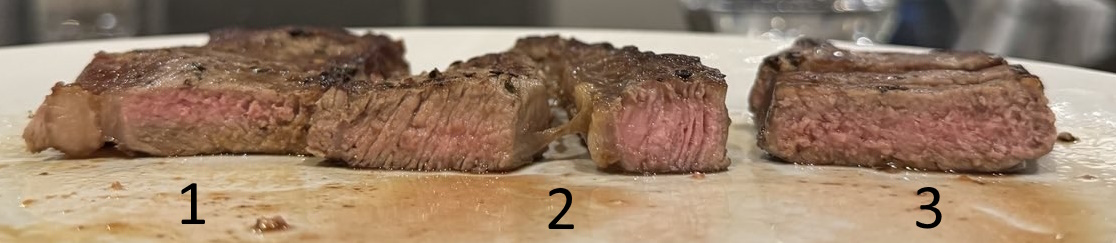
\includegraphics[width=0.9\textwidth]{./img/steak-side.jpeg}
		\caption{Top views and cross-sections of the steaks cooked in three different ways: (1) a single-flip pan sear, (2) a rapid-flip pan sear, and (3) a reverse sear.}
		\label{fig:steak}
	\end{figure}
	
	The trial (although it did only have a sample size of two) ordered the cooking methods (from best to worst) as: rapid-flip sear, reverse sear, single-flip sear. This was far from an accurate experiment, with many variables not controlled well, however it mostly agrees with my conclusions from the modelling. The only deviation was the reverse sear, which I believe was affected by not having a hot enough pan for the final sear, and overcooking it in the oven. The rapid-flip method also appeared to have more Maillard reaction take place, contrary to my modelling predictions. This could be somewhere that the modelling of steam would have an effect on.

\end{document}
